\documentclass{acm_proc_article-sp}

\usepackage{graphicx}% Include figure files
\usepackage{dcolumn}% Align table columns on decimal point
\usepackage{bm}% bold math
\usepackage{float}
\usepackage{array}
\usepackage{verbatim}
\usepackage{hyperref}% add hypertext capabilities
%\usepackage[mathlines]{lineno}% Enable numbering of text and display math
%\linenumbers\relax % Commence numbering lines
\usepackage[section]{placeins}
\usepackage{caption}
\usepackage{subcaption}

\usepackage{listings}
%\usepackage{footnote}
%\makesavenoteenv{table}
%\makesavenoteenv{table*}
%\makesavenoteenv{tabular}

\begin{document}

\title{Self-Organizing systems WS14 - Exercise 2\\
       Self-Organizing Maps}% Force line breaks with \\

\numberofauthors{2}
\author{
\alignauthor
Dragan Avramovski\\
       \email{e1426093@student.tuwien.ac.at}
\alignauthor
Richard Plangger\\
 \email{e1025637@student.tuwien.ac.at}
}

\date{\today}

\maketitle

\begin{abstract}
    This document summarizes our findings for the second exercise
    of the course self organizing systems at TU Wien.
\end{abstract}

\keywords{Self organizing systems, SOM }

\section{Wine dataset}

For our dataset we chose the ``wine-quality'' dataset from the UCI Machine Learning Repository~\cite{ucirepo}. 
Hereafter the dataset is called WQ.
It is data from wine variants of a Portuguese wine called ``Vino Verde''.
The data points the quality measure are physicochemical values measured
by sensors or tests. There is no information about the grape types,
wine brand, selling prices of the wine.
WQ has 12 different attributes and more than 6500 instances of red and white wine listed in the following enumeration:

\begin{itemize}
    \item Fixed acidity
    \item Volatile acidity
    \item Citric acid
    \item Residual sugar
    \item Chlorides
    \item Free sulfur dioxide
    \item Total sulfur dioxide
    \item Density
    \item pH
    \item Sulphates
    \item Alcohol
    \item Quality (A score between 0 and 10)
    \item Wine type (Red or white wine)
\end{itemize}

The data set contains two separate data files. One for white wine,
another for red wine. We merged the two together into a monolitic file,
and appending the wine type as a new attribute. $0$ denotes red wine, $1$ white wine.

The attribute quality is the only attribute that are human decided.
Each data entry has at least opinions of three different experts. This
sensory data is collected and the median the value included in the
dataset.

\section{Normalisation and data cleaning}

To get a feeling of the distribution of the data we used
WEKA to plot each attribute along its value range to visualise
density and the distribution.
Figure~\ref{fig:dist-alcohol} shows the distribution of the alcohol attribute. pH has
also a very similar distribution and both do not seem to have outliers.
For these two attributes we apply min/max scaling.

\begin{figure}
\centering
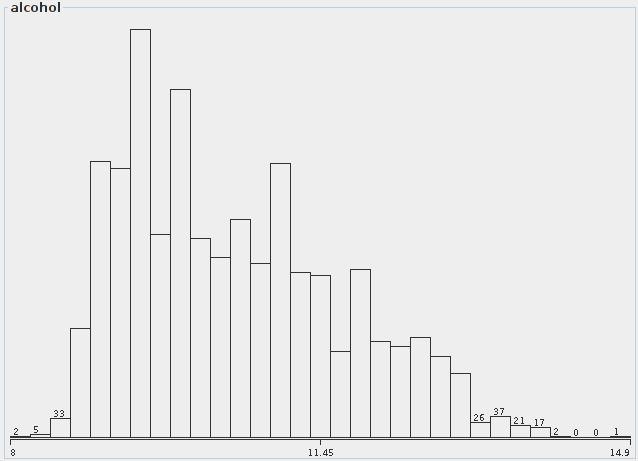
\includegraphics[width=0.6\linewidth]{img/dist-alcohol}
\caption{Data distribution of the alcohol attribute (not normalized)}
\label{fig:dist-alcohol}
\end{figure}


For Fixed/Volatile acidity and Total sulfur dioxide we apply Zero Mean Variance scaling. For these three we 
believe that the few outliers are features, not noise in the measurements.
For all others\footnote{Citri acid, Residual Sugar, Chlorides, Free/Total sulfur dioxide, Density, Sulphates}
we decided to exclude data samples with the outliers. The Table~\ref{tab:cutoff} shows the threshold after we drop
the data record. In Figure~\ref{fig:dist-citric-acid} a sample of the not normalized data is shown. A lot
of samples have a value to the left of the attribute range. Figure~\ref{fig:ndist-citric-acid} shows the
normalized attribute range.

\begin{figure}
\centering
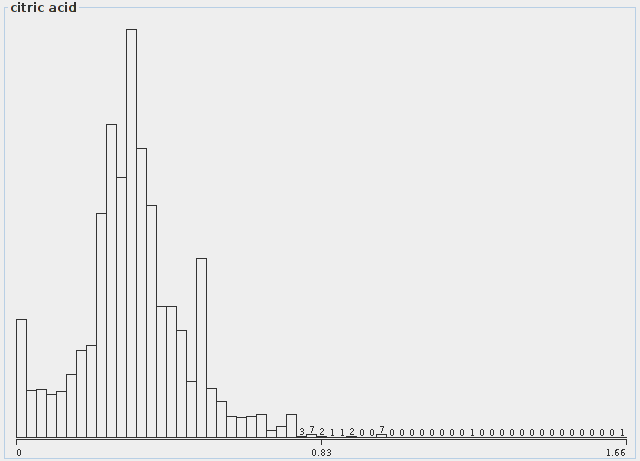
\includegraphics[width=0.6\linewidth]{img/dist-citric-acid}
\caption{Data distribution of the citric acid attribute (not normalized)}
\label{fig:dist-citric-acid}
\end{figure}

\begin{figure}
\centering
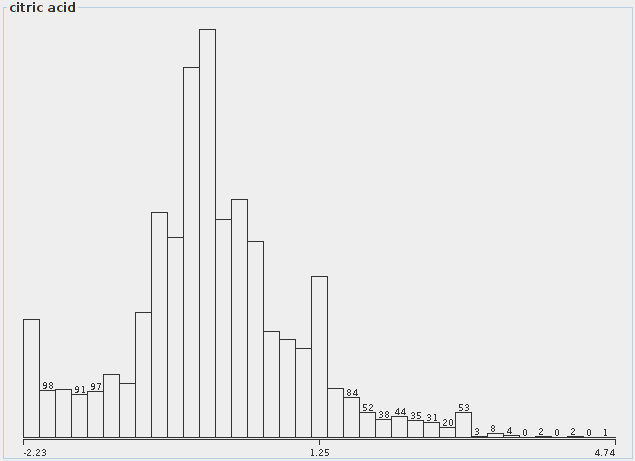
\includegraphics[width=0.6\linewidth]{img/ndist-citric-acid}
\caption{Data distribution of the citric acid attribute (normalized)}
\label{fig:ndist-citric-acid}
\end{figure}

\begin{table}
\centering
\begin{tabular}{l|c}
    Attribute & Cutoff \\
    \hline
    \hline
    Citri acid & 1.0 \\
    \hline
    Residual Sugar & 30.0 \\
    \hline
    Chlorides & 0.3 \\
    \hline
    Free sulfur dioxide & 150 \\
    \hline
    Density & 1.01 \\
    \hline
    Sulphates & 1.3 \\
\end{tabular}
\caption{Table that shows the cutoff for normalizations}
\label{tab:cutoff}
\end{table}

The total amount of rows that are filtered are 44 rows. This decreases the data set from 6497 instances to 6453.
We provide the original data samples in a file called ``wq.csv'', the samples that do not include quality and wine type
in ``wq-n-o.csv'' and the normalized data in ``wq-n.csv''.

\begin{comment}
In our automated script we used Python 2.7. To repeat the experiment we set the random seed to 0.
It cannot occur that one data sample of the original samples is included twice in the subsampled dataset.
\end{comment}
We also include the Python script called ``wine.py'' that can be invoked\footnote{Example: \$ python wine.py < wq.csv or 
\$ python wine.py 1500 < wq.csv} on the original dataset ``wq.csv'' to generate all files needed by the SOMToolbox.

\subsection{Classification}

In the original data set the attribute quality were used for classification. As we merged the white and red wine,
we additionally binned the quality into 3 bins: Poor-, Average- and High- quality. We did this, to reduce the possible
amount of classes (6 instead of approx. 14).
The data samples included in WQ covered a range from 3 to 9. Table~\ref{tab:quality-binning} shows the binning settings.
The bins are not equally distributed along the range, but we selected them by seeing the distribution in WEKA. Nearly
all bins should have an equal amount of samples associated to them.

\begin{table}
\centering
\begin{tabular}{l|c|c}
    Class & Quality Range & Class ID (red/white)\\
    \hline
    \hline
    Poorquality & $[0,5]$ & (0,1) \\
    \hline
    Averagequality & $[6,6]$ & (2,3) \\
    \hline
    Highquality & $[7,10]$ & (4,5) \\
    \hline
\end{tabular}
\caption{Shows the binning range for white and red wine}
\label{tab:quality-binning}
\end{table}

\subsection{Default settings}

If not noted otherwise the default parameter values are used for all quality measures and visualisations.
As an example the referent unit of the activity histogram is the default unit (0,0).

\section{Training the first SOM}

After we familiarized ourselves with the SOMToolbox we started by training a small
map. The initial settings for the ``Small Map'' are shown in Table~\ref{tab:settings}. 
The following list explains the settings shown in Table~\ref{tab:settings} in more detail.

\begin{itemize}
    \item $\alpha$ ... the learning rate
    \item $\sigma$ ... the neighbourhood radius
    \item $s_x$ ... size of the SOM grid on the x-axis
    \item $s_y$ ... size of the SOM grid on the y-axis
    \item $i$ ... the amount of iterations
\end{itemize}

For all of our experiments we prohibit the SOM Toolbox to normalize the data because we have
already done it previously.

\begin{table*}
\centering
\begin{tabular}{|l|c|c|c|c|c|c|}
    \hline
    Small Map & $\alpha = 0.75$ & $\sigma = 7$ & $s_x=5$ & $s_y=5$ & $i=1.500$ \\
    \hline
    Big Map & $\alpha = 0.75$ & $\sigma = 7$ & $s_x=50/30$ & $s_y=50/30$ & $i=1.500$ \\
    \hline
    Middle sized Map & $\alpha = 0.75$ & $\sigma = 7$ & $s_x=18$ & $s_y=18$ & $i=1.500$ \\
    \hline
    Rectangular mid sized Map & $\alpha = 0.75$ & $\sigma = 7$ & $s_x=20$ & $s_y=16$ & $i=1.500$ \\
    \hline
    Erroneous normalized Map & $\alpha = 0.75$ & $\sigma = 7$ & $s_x=14$ & $s_y=20$ & $i=1.500$ \\
    \hline
    Neighbourhood Small & $\alpha = 0.75$ & $\sigma = 1$ & $s_x=20$ & $s_y=16$ & $i=5.000$ \\
    \hline
    Neighbourhood Mid & $\alpha = 0.75$ & $\sigma = 5$ & $s_x=20$ & $s_y=16$ & $i=5.000$ \\
    \hline
    Neighbourhood Normal & $\alpha = 0.75$ & $\sigma = 10$ & $s_x=20$ & $s_y=16$ & $i=5.000$ \\
    \hline
    Neighbourhood Big & $\alpha = 0.75$ & $\sigma = 15$ & $s_x=20$ & $s_y=16$ & $i=5.000$ \\
    \hline
    Iterations 10 & $\alpha = 0.75$ & $\sigma = 10$ & $s_x=20$ & $s_y=16$ & $i=10$ \\
    \hline
    Iterations 50 & $\alpha = 0.75$ & $\sigma = 10$ & $s_x=20$ & $s_y=16$ & $i=50$ \\
    \hline
    Iterations 500 & $\alpha = 0.75$ & $\sigma = 10$ & $s_x=20$ & $s_y=16$ & $i=500$ \\
    \hline
    Iterations 10.000 & $\alpha = 0.75$ & $\sigma = 10$ & $s_x=20$ & $s_y=16$ & $i=10.000$ \\
    \hline
    Alpha 0.01 & $\alpha = 0.01$ & $\sigma = 10$ & $s_x=20$ & $s_y=16$ & $i=1.500$ \\
    \hline
    Alpha 0.45 & $\alpha = 0.45$ & $\sigma = 10$ & $s_x=20$ & $s_y=16$ & $i=1.500$ \\
    \hline
    Alpha 0.7 & $\alpha = 0.7$ & $\sigma = 10$ & $s_x=20$ & $s_y=16$ & $i=1.500$ \\
    \hline
    Alpha 0.99 & $\alpha = 0.99$ & $\sigma = 10$ & $s_x=20$ & $s_y=16$ & $i=1.500$ \\
    \hline
\end{tabular}
\caption{Settings for all of our experiments}
\label{tab:settings}
\end{table*}

\subsection{Small SOM}

We consider a grid of $5\times5$ units for our first 'very small SOM' experiment. WQ has more than 6000 entries.
This will result in many input samples grouped together to very few nodes. Our first trained
SOM is shown in Figure~\ref{fig:wine-small-hit-histogram} using the hit histogram visualization.
It can reveal dense areas on the map and in our opinion shows that the map size is too small.
We only have few units that are not fully colored in red, positioned in a vertical line and separating
the first 4 vertical units on the top left from the rest of the map. We conclude that there are
too many input samples are mapped to every unit in the SOM.

\begin{figure}
\centering
\begin{subfigure}[b]{0.45\linewidth}
    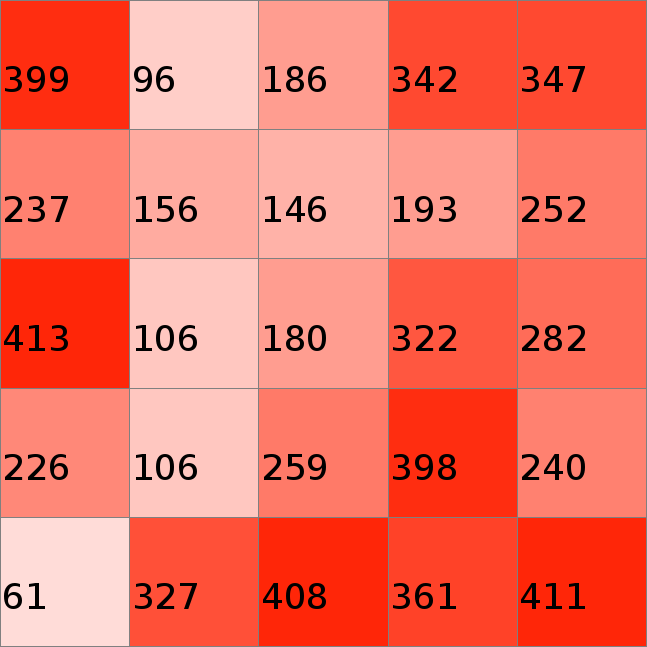
\includegraphics[width=\linewidth]{img/wine-small-hit-histogram}
    \caption{Hit histogram}
    \label{fig:wine-small-hit-histogram}
\end{subfigure}
\begin{subfigure}[b]{0.45\linewidth}
    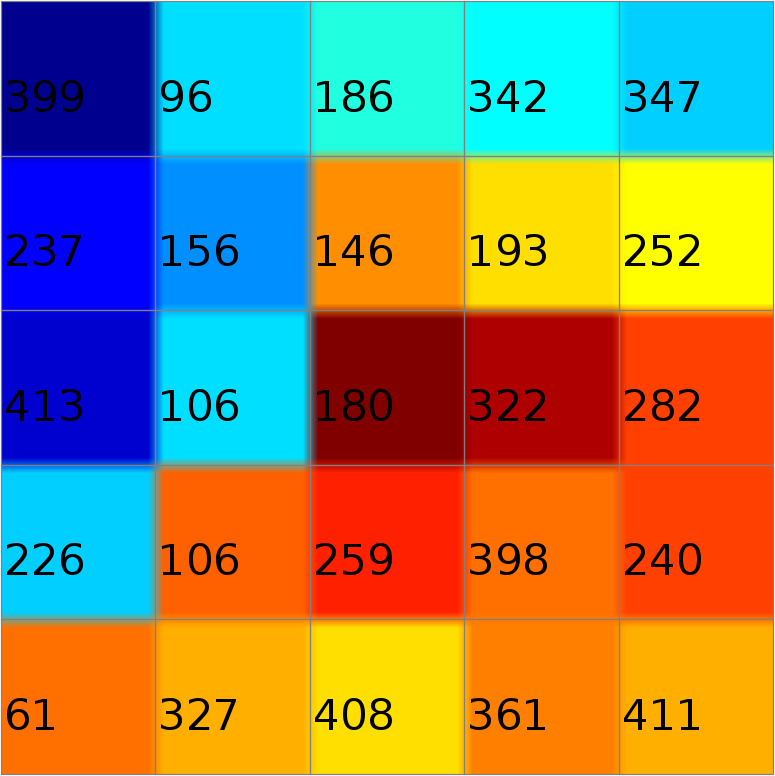
\includegraphics[width=\linewidth]{img/wine-small-p-matrix}
    \caption{P-Matrix Visualization}
    \label{fig:wine-small-p-matrix}
\end{subfigure}
\begin{subfigure}[b]{0.45\linewidth}
    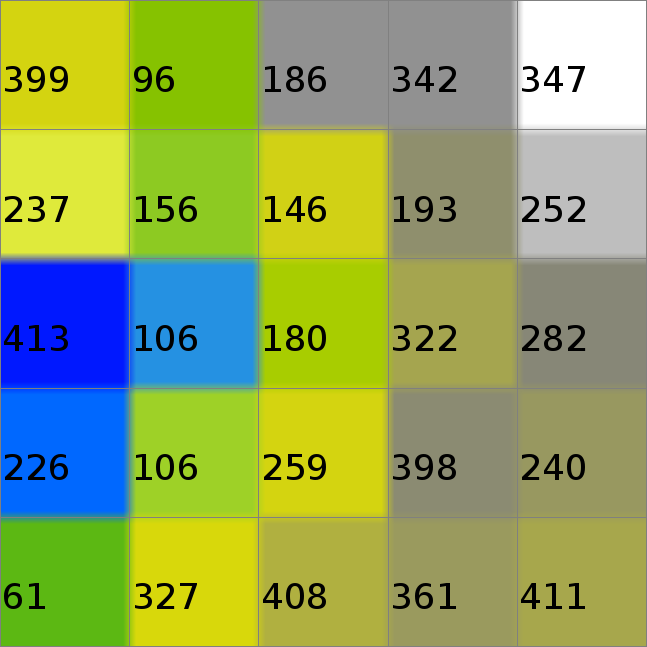
\includegraphics[width=\linewidth]{img/wine-small-activity-histogram}
    \caption{Activity histogram}
    \label{fig:wine-small-activity-histogram}
\end{subfigure}
\begin{subfigure}[b]{0.45\linewidth}
    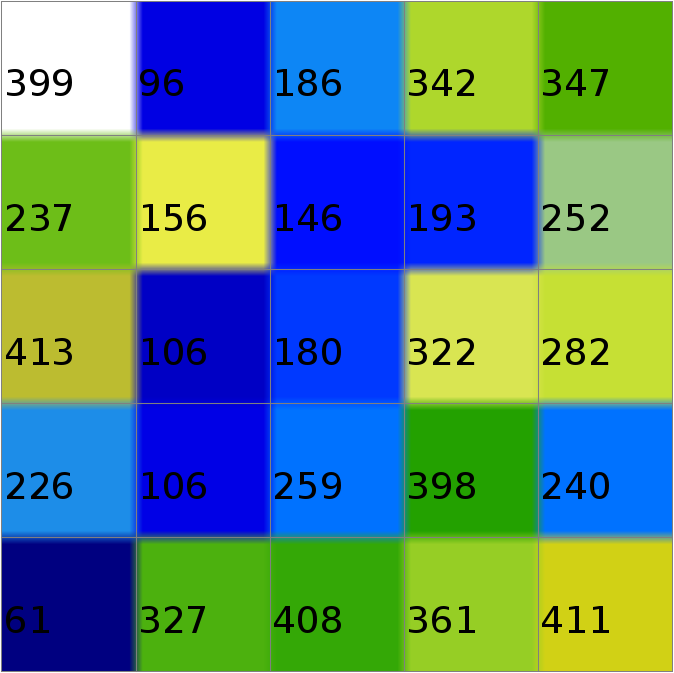
\includegraphics[width=\linewidth]{img/wine-small-quant-error}
    \caption{Quantization error}
    \label{fig:wine-small-quant-error}
\end{subfigure}
    \caption{SOM $5\times5$ SOM}
\end{figure}

Another visualization hint for dense areas is the P-Matrix. It is shown in Figure~\ref{fig:wine-small-p-matrix} using
the default settings. We see that there are dense areas to the bottom right of the map and there are lesser
dense areas to the top left of the map.
By increasing the P-radius from 3 to 5 the map nearly turns into one big red pixel.
Comparing it to Figure~\ref{fig:wine-small-hit-histogram} it shows that there are many input samples densly packed
onto the lower right grid of the map. We assume that by increasing the SOM size, this data will be distributed much better. Another assumption is that a rectangular map will fit the data better as the units seem to spread into a similar shape.

We also present the Activity Histogram of our small SOM in Figure~\ref{fig:wine-small-activity-histogram}.
Interesting is the blue part on the mid left that is separated by a slight green/yellow.
On the bottom right we again find a very dense area because of the grayish/yellow color. This this matches
well with the P-Matrix visualization. Judging from the Activity Histogram there are 2 very distinct clusters
and maybe one cluster that is very intermixed (green/yellow). This could either be that the
red and white wine are very distinct or two subranges of the quality are dominated by ranges of the input.

\subsection{Quality measurements}

In the following we take a look at some quality measures available in SOMToolbox.
If not noted otherwise the default SOM parameter values are used for all quality measures and visualisations.
First we compare the Quantization Error (QE) and the Mean Quantization Error (MQE) shown in
Figure~\ref{fig:wine-small-quant-error} and~\ref{fig:wine-small-mean-quant-error} respectivley.
We already noted that the lower right is a very dense area. In the MQE these units have a very low
MQE rate thus they are colored blue. In the QE Figure the values are much more scattered. In
the top left it has a very high value thus it seems that there is an area that is not that dense
and has many items with a long distance. This we also can confirm using the MQE, because the division
by the nodes does not set a low value the value in MQE. It also reveals that there is potentially even a more sparse
region as the node at position (1,1) in MQE shows.

\begin{figure}
\centering
\begin{subfigure}[b]{0.45\linewidth}
    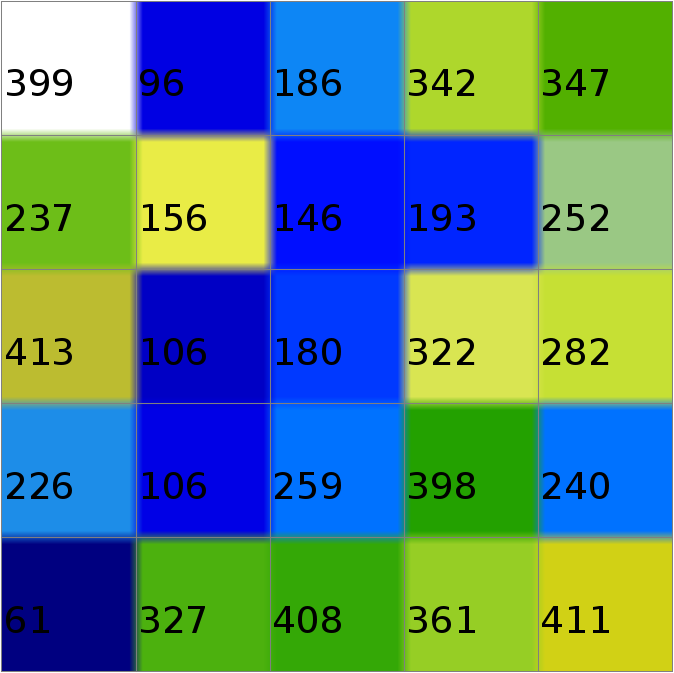
\includegraphics[width=\linewidth]{img/wine-small-quant-error}
    \caption{Quantization error}
    \label{fig:wine-small-quant-error}
\end{subfigure}
\begin{subfigure}[b]{0.45\linewidth}
    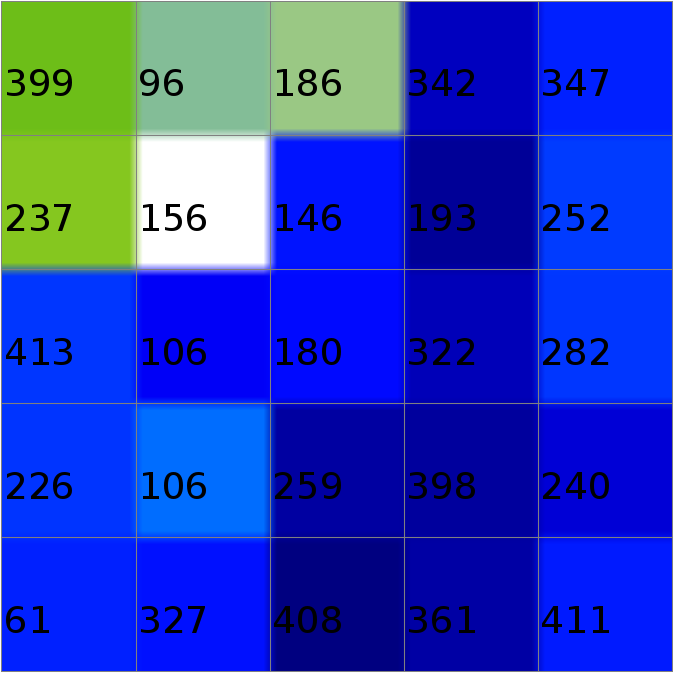
\includegraphics[width=\linewidth]{img/wine-small-mean-quant-error}
    \caption{Mean quantization error}
    \label{fig:wine-small-mean-quant-error}
\end{subfigure}
\begin{subfigure}[b]{0.45\linewidth}
    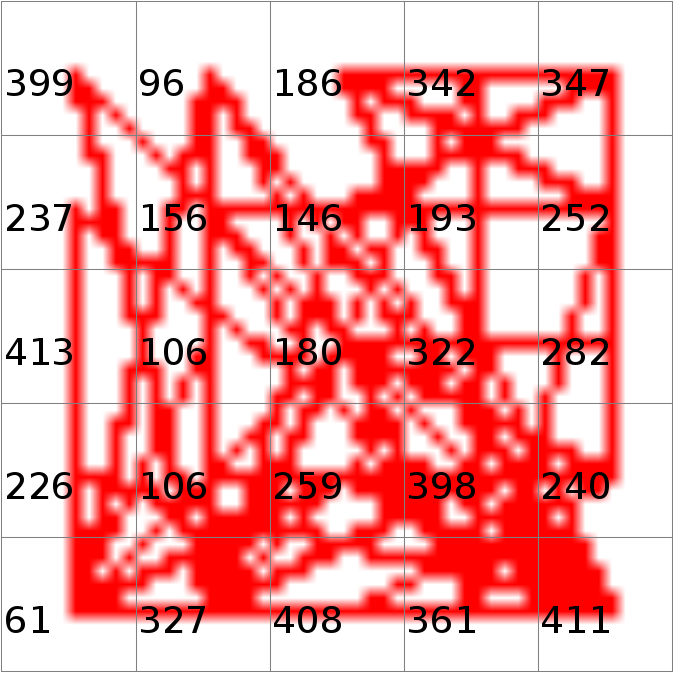
\includegraphics[width=\linewidth]{img/wine-small-dist-sqrt-2}
    \caption{Distortion ($\sqrt{2}$)}
    \label{fig:wine-small-dist-sqrt-2}
\end{subfigure}
\begin{subfigure}[b]{0.45\linewidth}
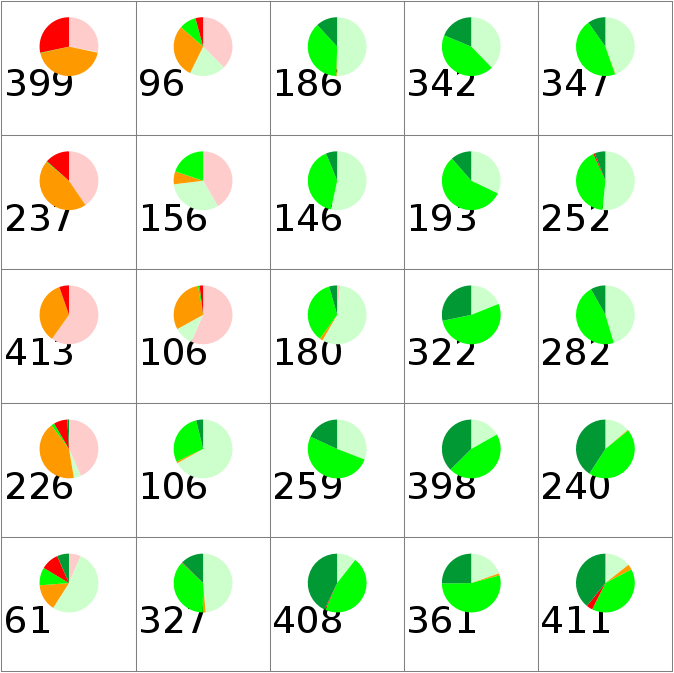
\includegraphics[width=\linewidth]{img/wine-small-pie-cls}
\caption{Classes}
\label{fig:wine-small-pie-cls}
\end{subfigure}
\caption{SOM $5\times5$}
\end{figure}

The map is also very distorted which is shown in Figure~\ref{fig:wine-small-dist-sqrt-2}.
When comparing this to a better train map (such as the sample of Iris dataset), it is
really distorted. Given the number of values mapped to the nodes, the distortion and
high QE we conclude current SOM size is to small and it is very hard to discover the shape of the data.

To finish the examination of this far to small map we show the class distribution amongst the map.
At first it surprised us that the splitting is done quite evenly between red and
white wine. Giving this a second thought it is clear that they must be more easily separatable.
White and red wine have very different characteristics in sugar, acid, etc. 
White wine is colored green (light green is poor quality, green is average quality and dark green is high quality) and
red wine is colored red(light for poor quality, orange for average quality and dark for high quality).

What we also have seen in the class distribution is that white wine has far more data samples
than the red wine. Thus we apply subsampling of white wine input samples.
We reduce the dataset to around 1500 red and 1500 white wine samples.
We use a random seed of 0 in our export script to repeat this experiment.

\section{A very big SOM}

Now we would like to examine the data in a very big SOM. The settings are displayed
in~\ref{tab:settings}. Our assumption is that it is too big if we have less than 3
samples per SOM unit.

To find out if the SOM is too big we take a look at the QE (Figure ~\ref{fig:wine-big-quant-error}) and MQE (Figure~\ref{fig:wine-big-mean-quant-error}) quality measurements.
The first thing we noticed is the huge number of interpolating/empty units on the map. By comparing QE and MQE we noticed that there is not
a significant differance in the color coding. This is caused by fact that map is too big and only a small number of samples
are mapped to the units.
At this point we immediatly stopped to evaluate this huge SOM and decreased the size to $30\times30$. The main reason was that we had problems
with the SOM Toolbox to display various visualizations. Even the $30\times30$ SOM confirms our assumption that big sized SOMs have
many interpolating units. The picture of the QE and MQE are quite the same but only with fewer nodes.

\begin{figure}
\centering
\begin{subfigure}[b]{0.45\linewidth}
    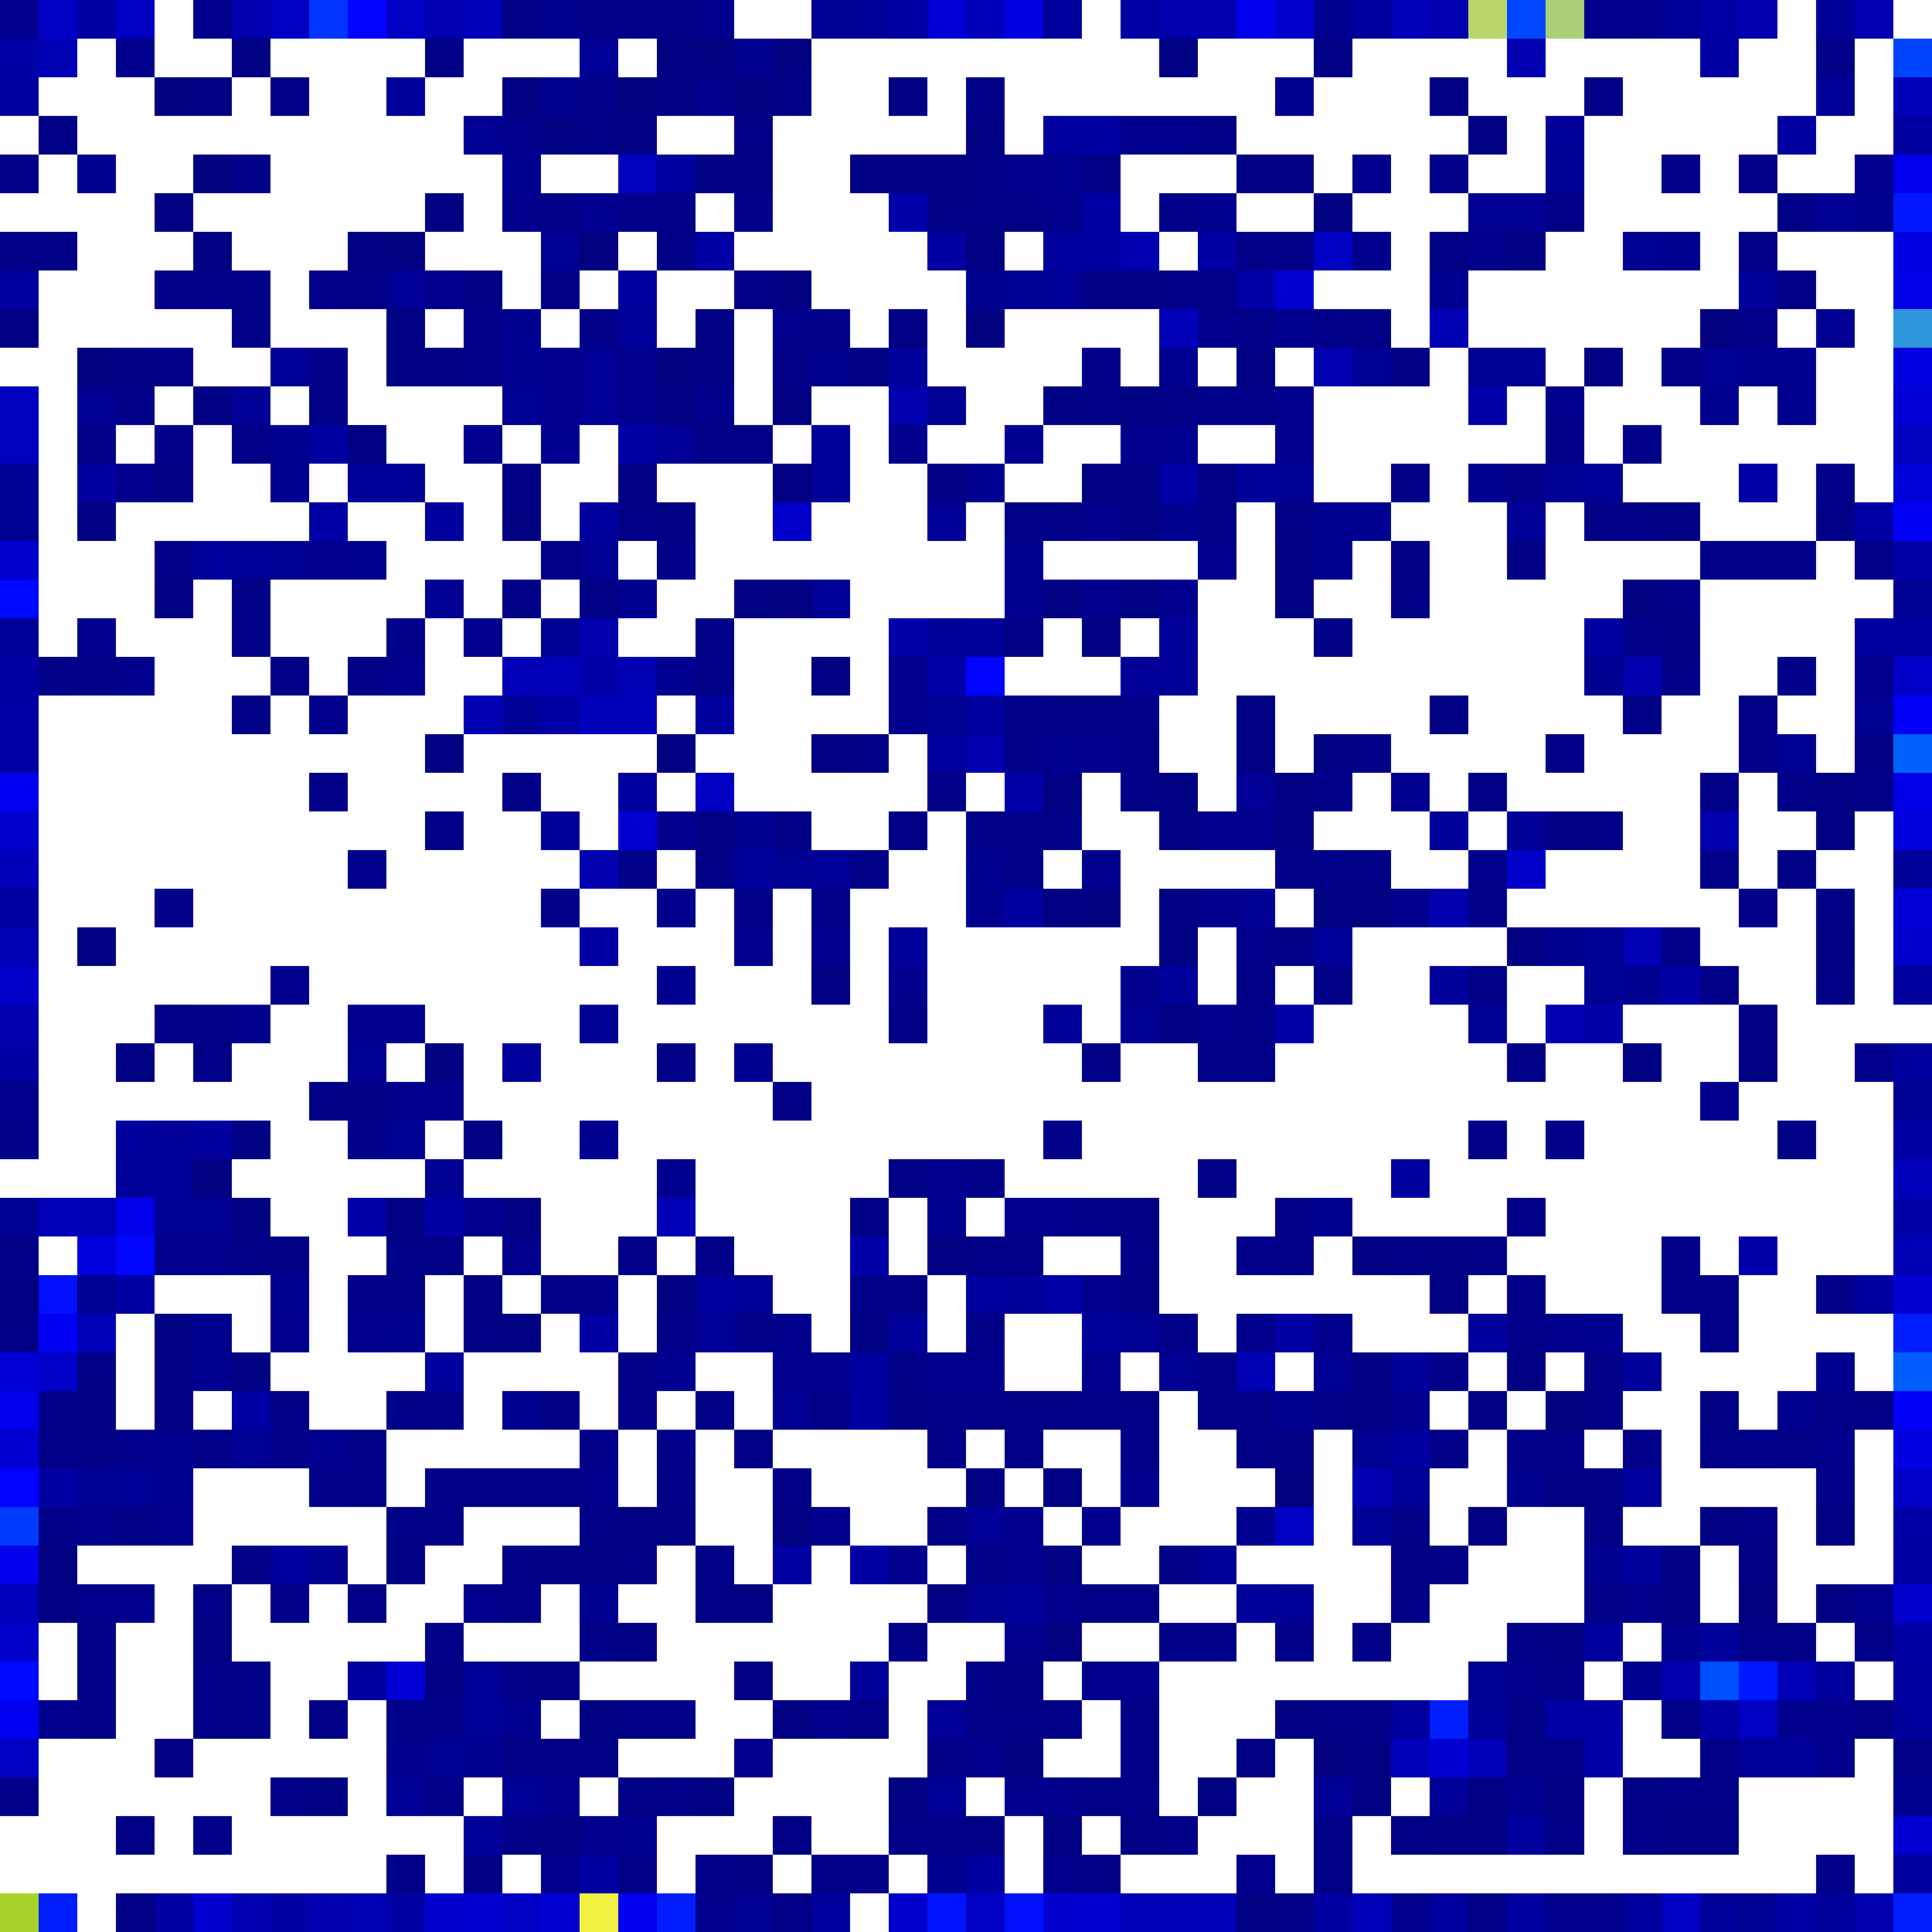
\includegraphics[width=\linewidth]{img/wine-big-quant-error}
    \caption{Quantisation error}
    \label{fig:wine-big-quant-error}
\end{subfigure}
\begin{subfigure}[b]{0.45\linewidth}
    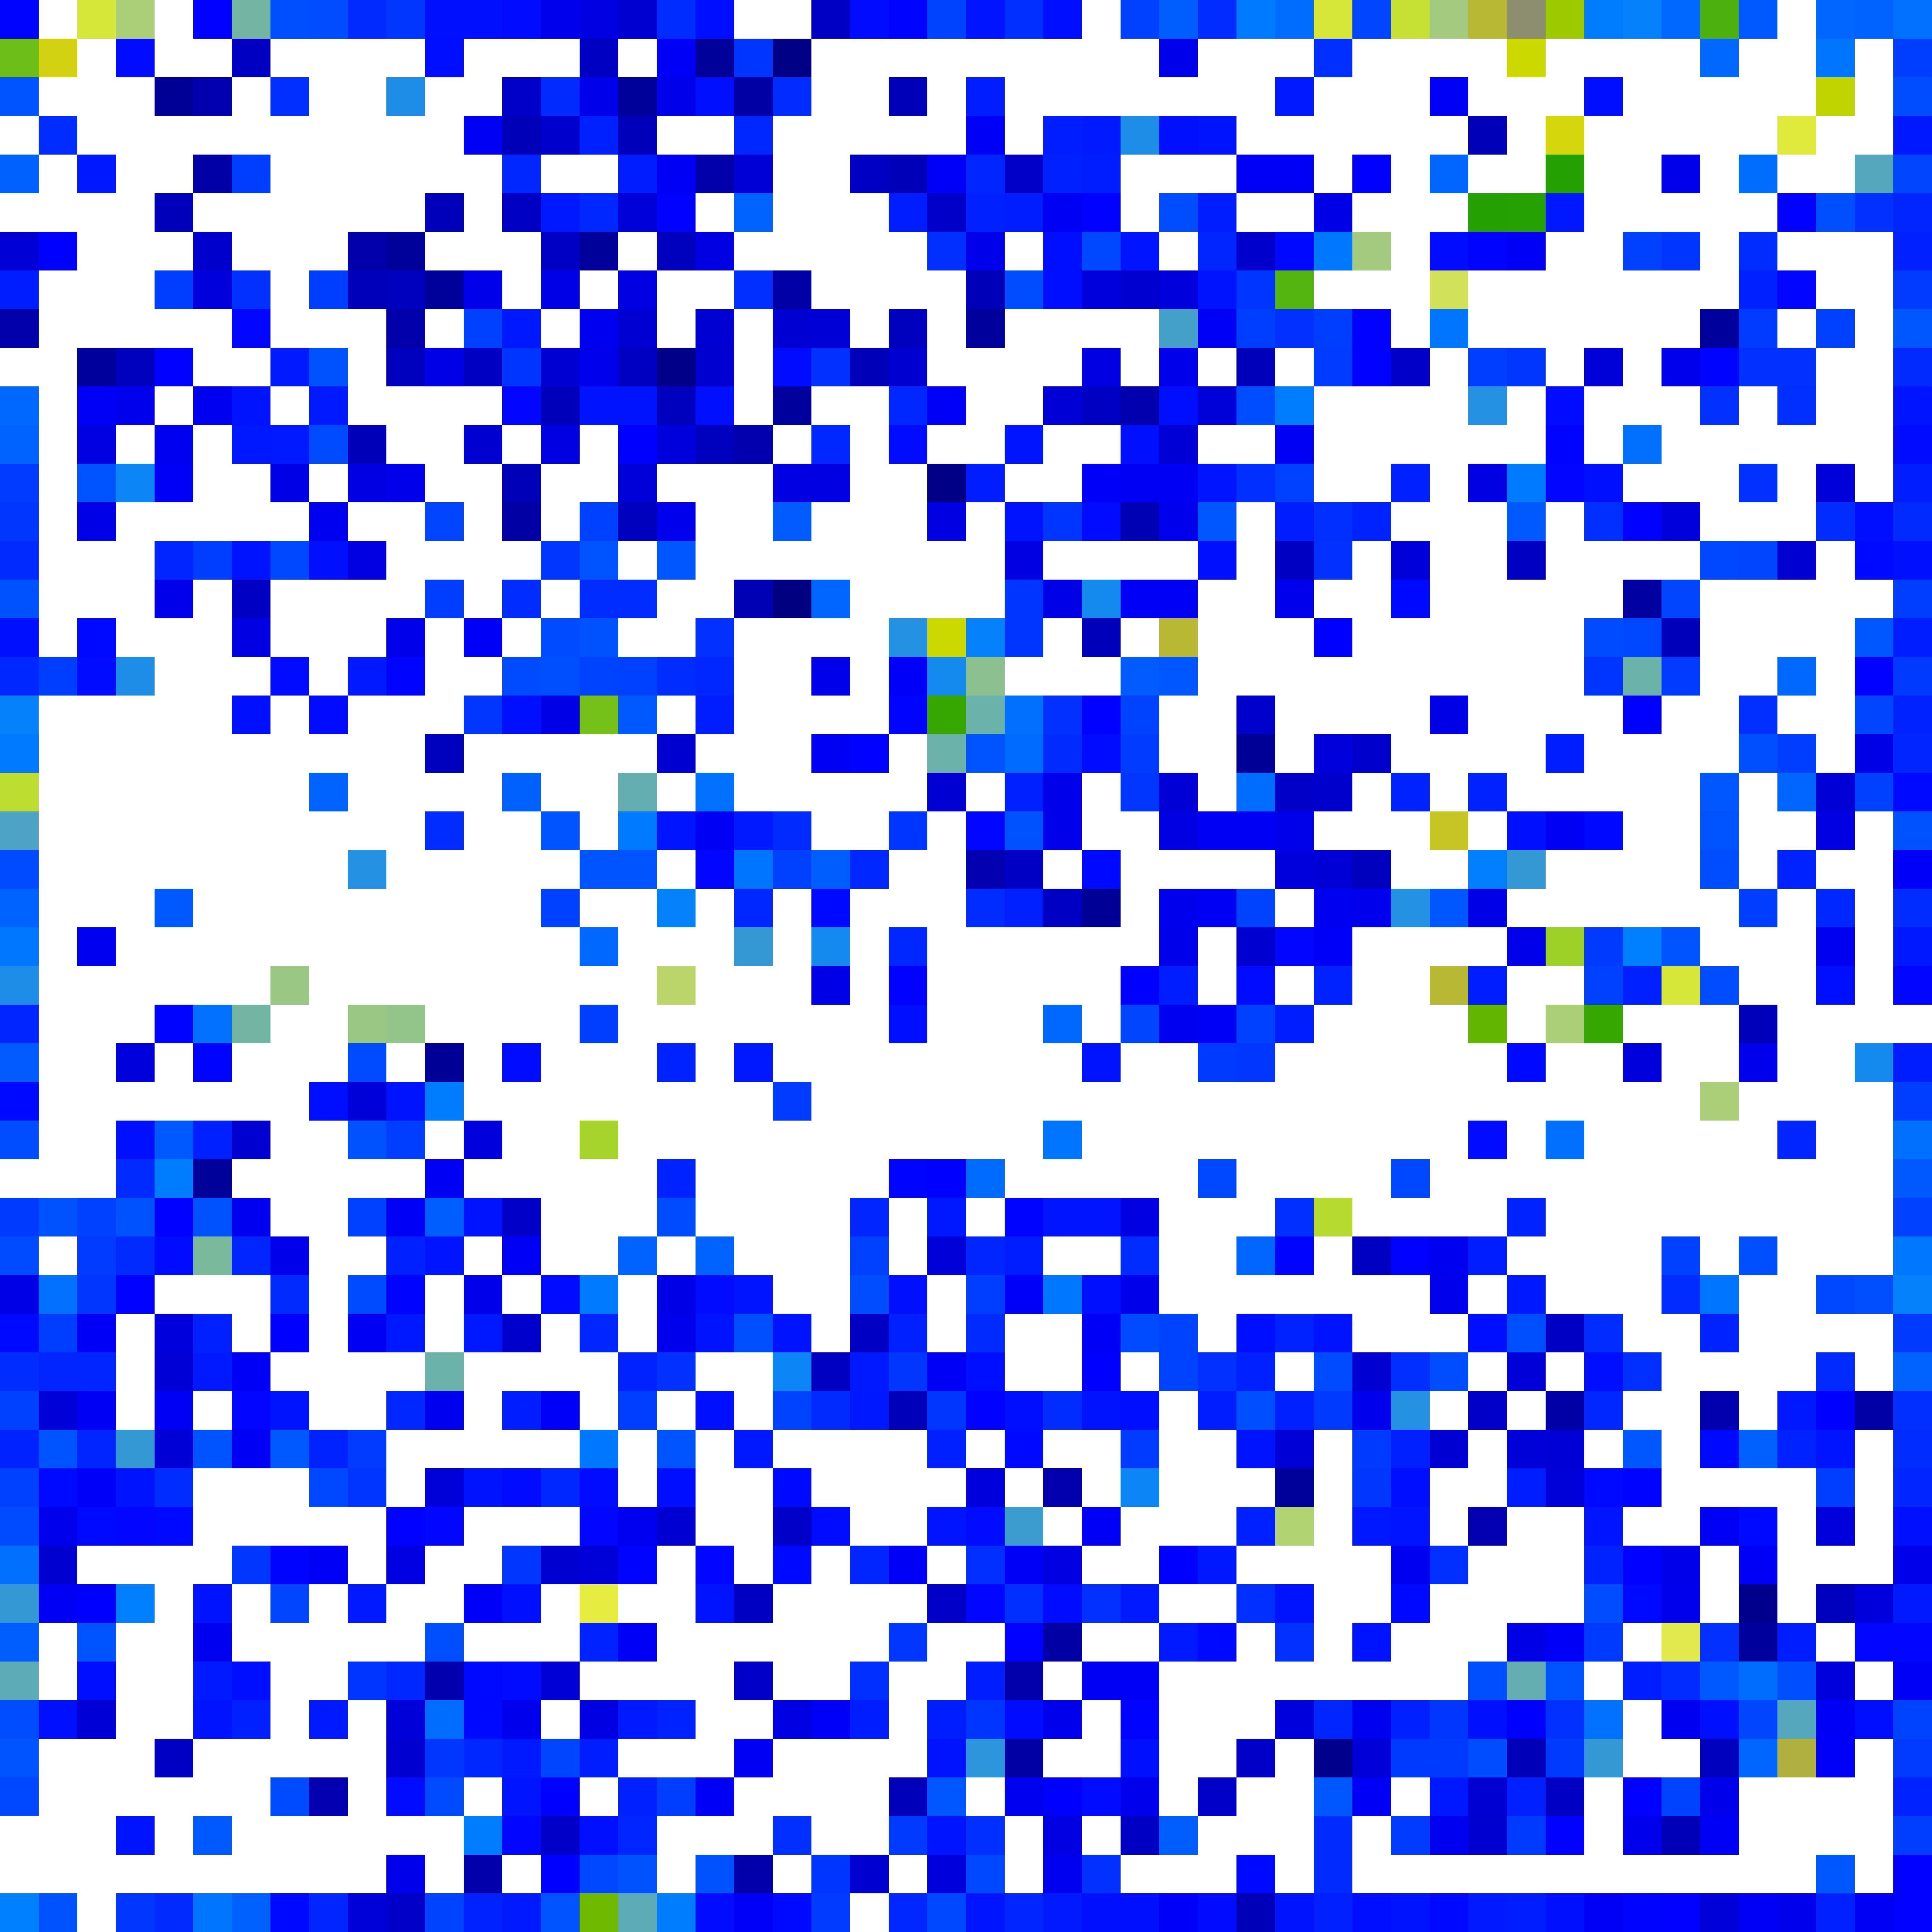
\includegraphics[width=\linewidth]{img/wine-big-mean-quant-error}
    \caption{Quantisation error}
    \label{fig:wine-big-mean-quant-error}
\end{subfigure}
\caption{SOM $50\times50$}
\end{figure}

\begin{figure}
\begin{subfigure}[b]{0.45\linewidth}
    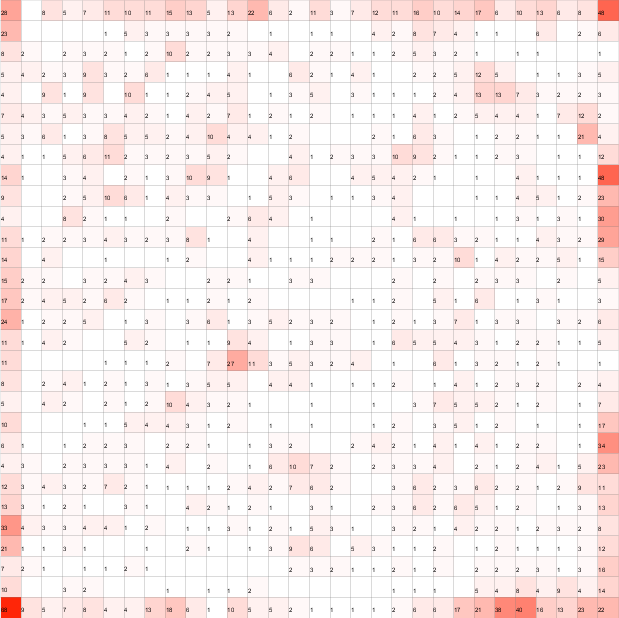
\includegraphics[width=\linewidth]{img/wine-big-hit-histogram}
    \caption{Hit histogram}
    \label{fig:wine-big-hit-histogram}
\end{subfigure}
\begin{subfigure}[b]{0.45\linewidth}
    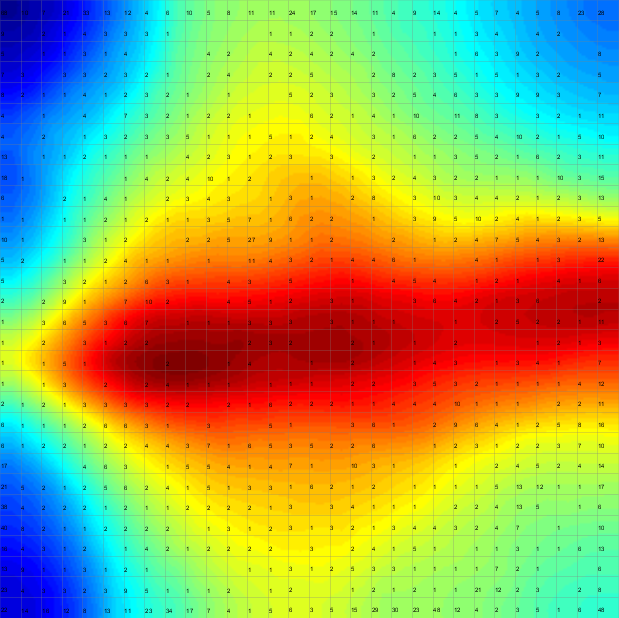
\includegraphics[width=\linewidth]{img/wine-big-p-matrix}
    \caption{P-Matrix visualization}
    \label{fig:wine-big-p-matrix}
\end{subfigure}
\begin{subfigure}[b]{0.45\linewidth}
    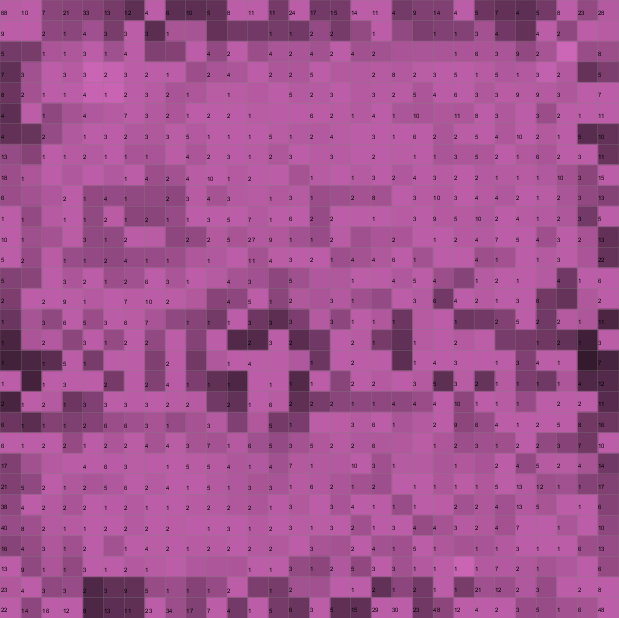
\includegraphics[width=\linewidth]{img/wine-big-topo-product}
    \caption{Topographic product}
    \label{fig:wine-big-topo-product}
\end{subfigure}
\begin{subfigure}[b]{0.45\linewidth}
    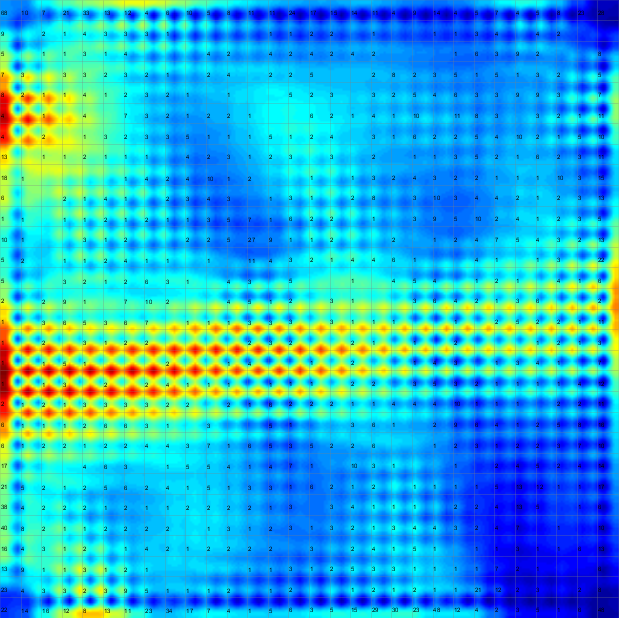
\includegraphics[width=\linewidth]{img/wine-big-u-matrix}
    \caption{U-Matrix}
    \label{fig:wine-big-u-matrix}
\end{subfigure}
\begin{subfigure}[b]{0.45\linewidth}
    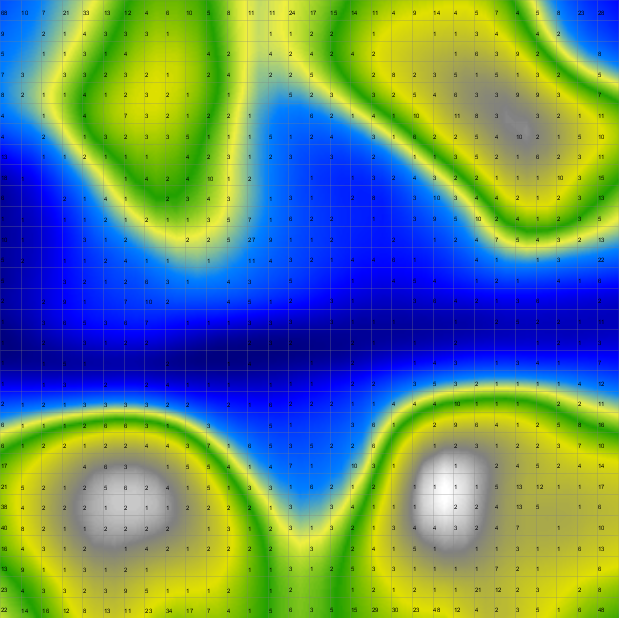
\includegraphics[width=\linewidth]{img/wine-big-smoothed-data-histogram}
    \caption{SDH}
    \label{fig:wine-big-smoothed-data-histogram}
\end{subfigure}
\begin{subfigure}[b]{0.45\linewidth}
    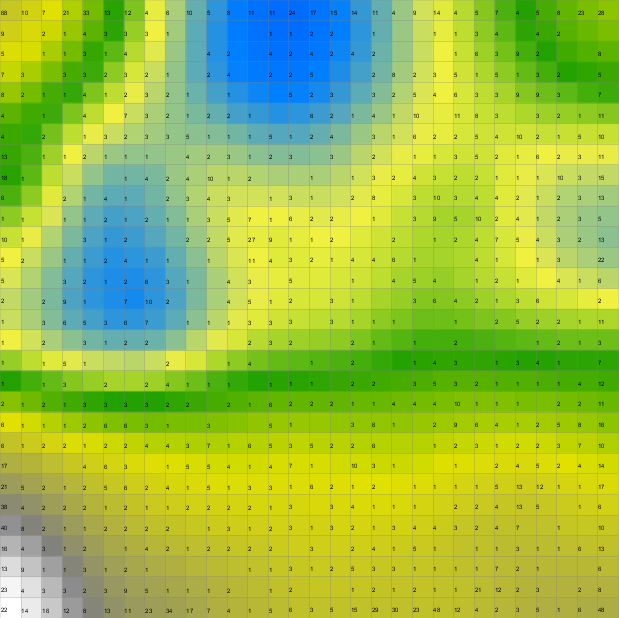
\includegraphics[width=\linewidth]{img/wine-big-activity-histogram}
    \caption{Activity histogram}
    \label{fig:wine-big-activity-histogram}
\end{subfigure}
\caption{SOM $30\times30$}
\end{figure}

We assume that the hit histogram of the $50\times50$ SOM should not have a lot of red spots.
Using the hit histogram of the smaller big SOM ($30\times30$) shown in Figure~\ref{fig:wine-big-hit-histogram} we notice that very light
colors which indicates that few or none input samples are mapped to the SOM nodes.

In Figure~\ref{fig:wine-big-p-matrix} we se a huge red spot in the center of the map. This indicates that
the data is very dense at this area. Comparing it to the small SOM P-Matrix there is this dense area
in the center. The difference is that the dense area is to the center right and not to the bottom right as assumed with
the small one.

The last quality measure we apply for this map is the topographic product.
We used a setting of $k=1$. The visualisation reveals a distortion in the
SOM borders and a horizontal line of distortion in the center of the map.
When increasing the number of neighbours ($k$) we still see the distortion
we mentioned earlier.

In the Figure~\ref{fig:wine-big-u-matrix} we show the U-Matrix visualization.
It reveals the possible cluster bounderies. We have many coherent regions/valleys located in
the upper and lower parts of the map. They are separated by a horizontal mountain regions
or high values in the center which depict the possible cluster boundaries.

The potential cluster boundaries are displayed in the SDH\footnote{Smoothed data histogram} visualization in Figure~\ref{fig:wine-big-smoothed-data-histogram}.

In addition, the Activity Histogram in Figure~\ref{fig:wine-big-activity-histogram} shows possible
topology violations especially in the upper cluster where the blue area is separated by green.
Thus we observe that a gradient of the weight vectors measured in distance is not present. 

The analysed visualizations/quality measures depict that we SOM is oversized.
In the following we will try to approximate a better size.

\section{Normal SOM}

In the following we show a mid sized map. Parameters are included in the Table~\ref{tab:settings}.
On the first view of QE in Figure~\ref{fig:wine-mid-quant-error} and MQE~\ref{fig:wine-mid-mean-quant-error} we see
that there are three interpolating units. Comparing the two we notice that the distant data samples are
mapped to the units located along the a horizontal line in the center or the potential cluster boundaries.
The U-Matrix in Figure~\ref{fig:wine-mid-u-matrix} reveals the cluster boundaries shown with high mountain values
along the line mentioned earlier.

Again we used the SDH visualization. In the earlier settings we used a smoothing factor of 149. We decreased it to
115 and managed to separate the two main clusters shown in Figure~\ref{fig:wine-mid-smoothed-data-histogram}.

There are potential topology violations located in the upper cluster. We see this in Figure~\ref{fig:wine-mid-activity-histogram}.
Similar to the the big SOM there are three blue areas separated by green an yellow.
By observing the neighbourhood graph shown in Figure~\ref{fig:wine-mid-radius-neighbourhood-graph} with a radius of 0.4, we notice three red lines connecting the blue areas.


\begin{figure}
\centering
\begin{subfigure}[b]{0.45\linewidth}
    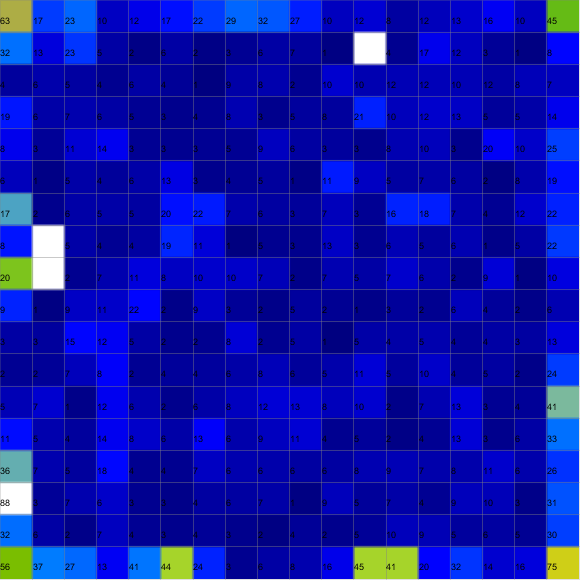
\includegraphics[width=\linewidth]{img/wine-mid-quant-error}
    \caption{Quantisation error}
    \label{fig:wine-mid-quant-error}
\end{subfigure}
\begin{subfigure}[b]{0.45\linewidth}
    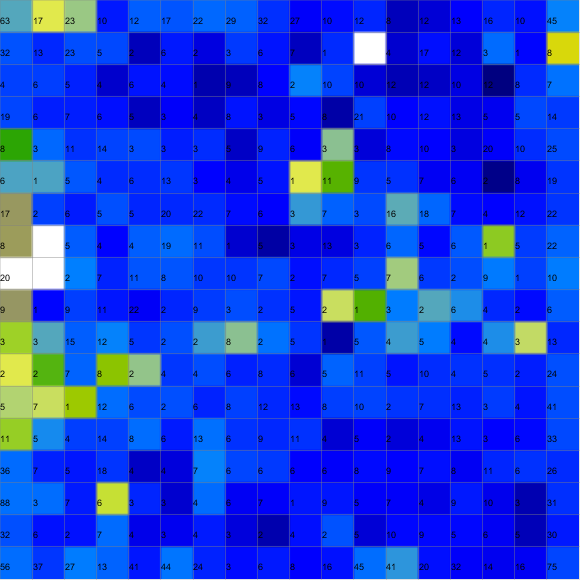
\includegraphics[width=\linewidth]{img/wine-mid-mean-quant-error}
    \caption{Mean quantisation error}
    \label{fig:wine-mid-mean-quant-error}
\end{subfigure}
\begin{subfigure}[b]{0.45\linewidth}
    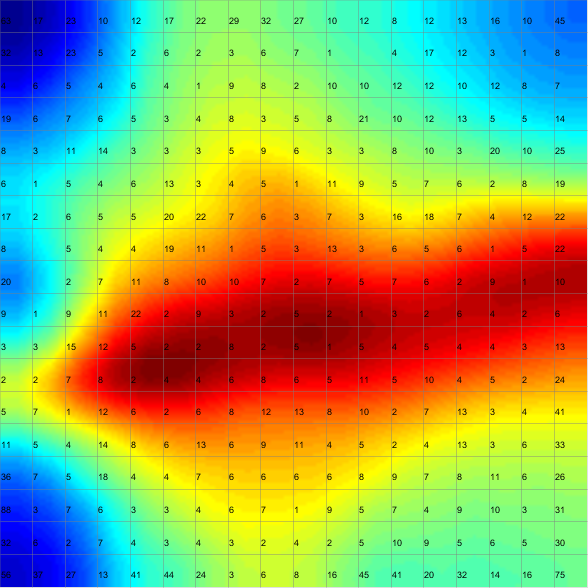
\includegraphics[width=\linewidth]{img/wine-mid-p-matrix}
    \caption{P-Matrix visualization}
    \label{fig:wine-mid-p-matrix}
\end{subfigure}
\begin{subfigure}[b]{0.45\linewidth}
    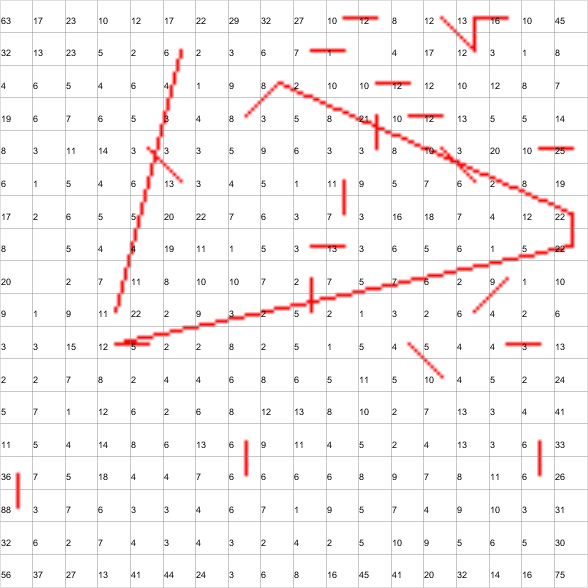
\includegraphics[width=\linewidth]{img/wine-mid-radius-neighbourhood-graph}
    \caption{Neighbourhood graph}
    \label{fig:wine-mid-radius-neighbourhood-graph}
\end{subfigure}
\begin{subfigure}[b]{0.45\linewidth}
    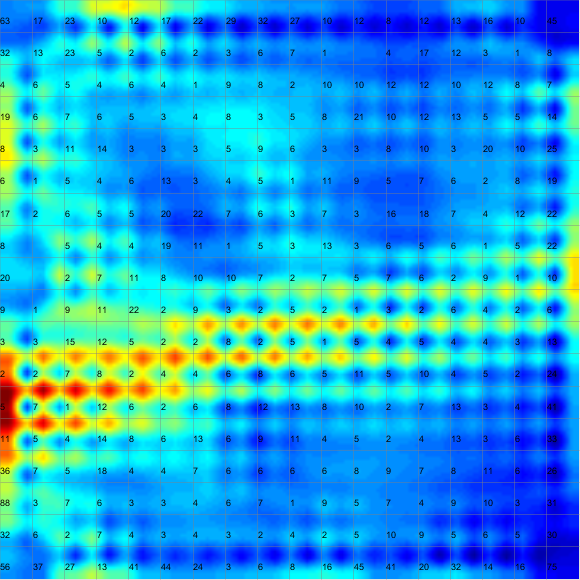
\includegraphics[width=\linewidth]{img/wine-mid-u-matrix}
    \caption{U-Matrix}
    \label{fig:wine-mid-u-matrix}
\end{subfigure}
\begin{subfigure}[b]{0.45\linewidth}
    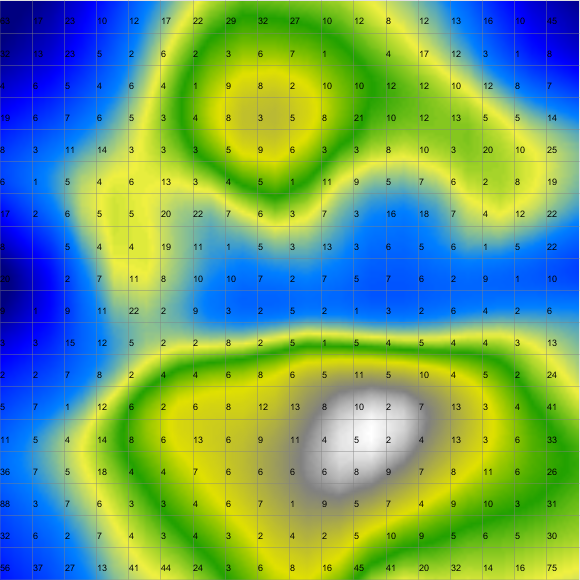
\includegraphics[width=\linewidth]{img/wine-mid-smoothed-data-histogram}
    \caption{SDH}
    \label{fig:wine-mid-smoothed-data-histogram}
\end{subfigure}
\begin{subfigure}[b]{0.45\linewidth}
    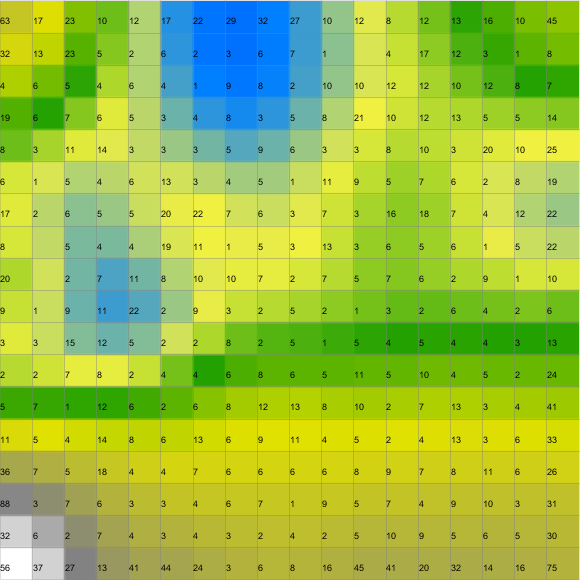
\includegraphics[width=\linewidth]{img/wine-mid-activity-histogram}
    \caption{Activity histogram}
    \label{fig:wine-mid-activity-histogram}
\end{subfigure}
\caption{SOM $18\times18$}
\end{figure}

\section{SOM random Initialization. Different Seed values}

As discovered in the previous analysis, the square SOM shown in Figure~\ref{fig:wine-mid-activity-histogram} contains critical Topology violations in the right area of the map. We tried to improve the mapping quality by training a mid sized SOM with rectangular structure and as shown on the Activity histograms in Figure~\ref{fig:wine-newmid-activity-histogram-seed} we managed to merge a group of similar weight vectors colored with blue in one area instead of being separated by green weight vectors as seen in the square SOM.

The rectangular SOM was trained with the default initial parameters as shown in Table Table~\ref{tab:settings}. Further to our analysis, we trained two additional SOMs with identical initial parameters but with different random initializations. The distinction in the initialization was done by specifying different seed values. As noted before, we discovered two main clusters and by observing the Activity Histogram in Figure~\ref{fig:wine-newmid-activity-histogram-seed} we notice the movement of these clusters. For $s = 1$ the right cluster is weak but as we increase the seed values to $s = 7$ we notice clearer definition of the blue area. Further more for $s = 55$ we observe a complete cluster shift.

The U-Matrices shown on Figure~\ref{fig:wine-newmid-u-matrix-seed} show that for $s = 1$ the cluster boundaries are vertical but not clearly defined. For $s = 7$ they are adjusted and clear whereas for $Seed = 55$ we observe a complete cluster boundaries shift into a horizontal position. 

New discoveries of the clusters shift are revealed by the Radius based Neighbourhood graphs by observing graphs with different radius values $r = 0.5$ shown in Figure~\ref{fig:wine-newmid-radius-neighbourhood-graph--r-05-seed}; $r= 0.8$ shown in Figure~\ref{fig:wine-newmid-radius-neighbourhood-graph--r-08-seed} and $r = 1$ shown in Figure~\ref{fig:wine-newmid-radius-neighbourhood-graph--r-10-seed}. 
For $s = 55$ the rotation of the cluster boundaries is confirmed. We notice one more smaller inner cluster shift for $s = 7$ and radius value of $r = 0.8$ shown on Figure~\ref{fig:wine-newmid-radius-neighbourhood-graph--r-08-seed} (b) and $r = 1$ shown on Figure~\ref{fig:wine-newmid-radius-neighbourhood-graph--r-10-seed} (b). The dense area of the Right cluster is moved to the lower right area of the SOM. Additional finding is that for $s = 1$ and $r = 0.5$ as shown in Figure~\ref{fig:wine-newmid-radius-neighbourhood-graph--r-05-seed}(a) we observe parallel lines which are indicators of Topology Violations.

\begin{figure}
\centering
    \centering
    \begin{subfigure}[b]{0.30\linewidth}
        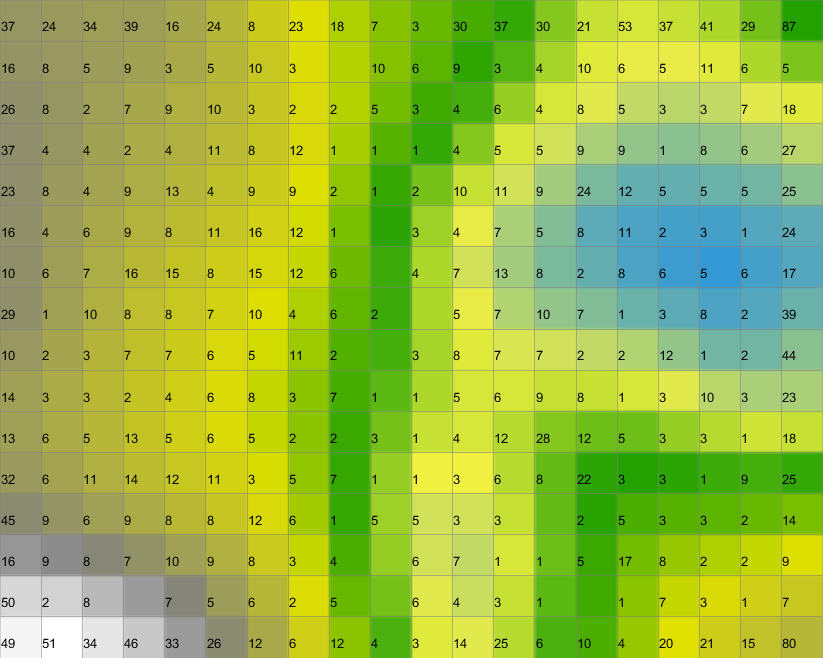
\includegraphics[width=\linewidth]{img/wine-newmid-activity-histogram-seed-1}
        \caption{$s=1$}
        \label{fig:wine-newmid-activity-histogram-seed-1}
    \end{subfigure}
    \begin{subfigure}[b]{0.30\linewidth}
        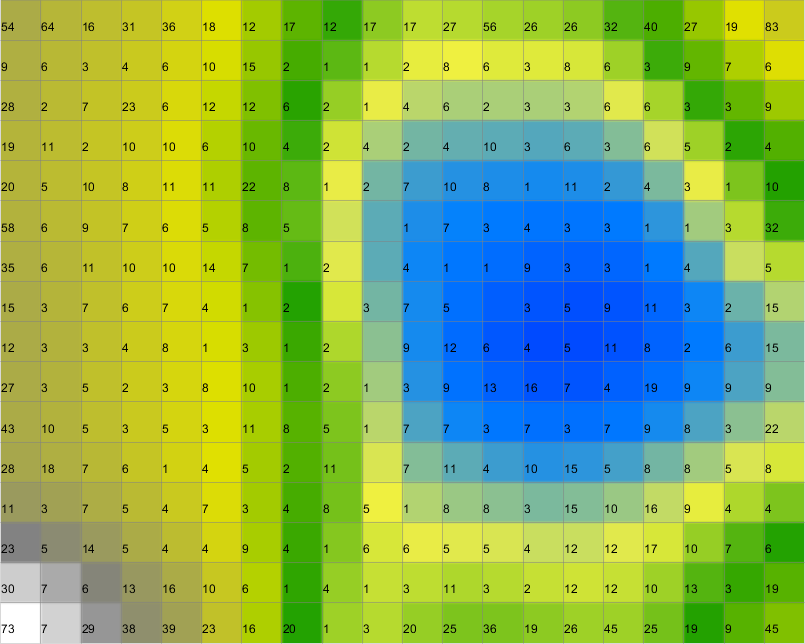
\includegraphics[width=\linewidth]{img/wine-newmid-activity-histogram-seed-7}
        \caption{$s=7$}
        \label{fig:wine-newmid-activity-histogram-seed-7}
    \end{subfigure}
    \begin{subfigure}[b]{0.30\linewidth}
        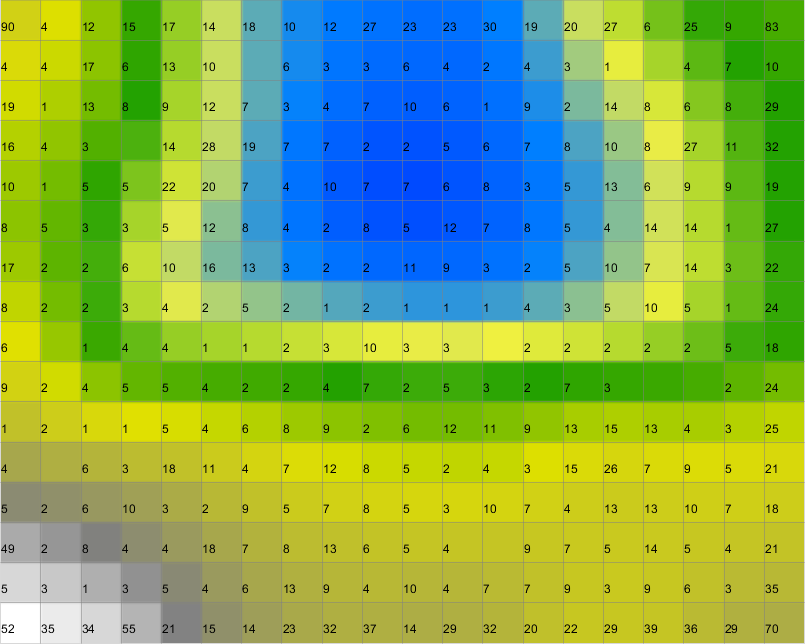
\includegraphics[width=\linewidth]{img/wine-newmid-activity-histogram-seed-55}
        \caption{$s=55$}
        \label{fig:wine-newmid-activity-histogram-seed-55}
    \end{subfigure}
    \caption{SOM ($20\times16$) Activity histogram with different seed values $s$}
    \label{fig:wine-newmid-activity-histogram-seed}
\end{figure}

\begin{figure}
\centering
    \centering
    \begin{subfigure}[b]{0.30\linewidth}
        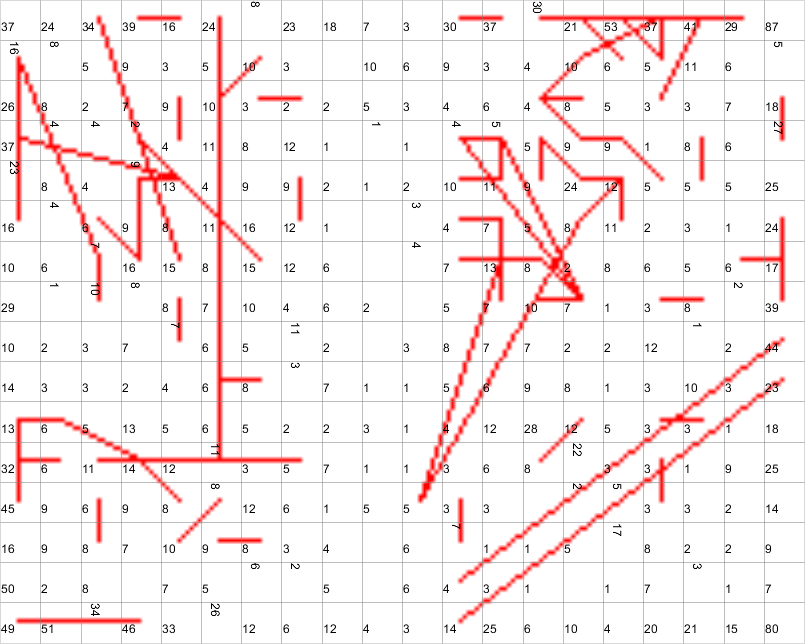
\includegraphics[width=\linewidth]{img/wine-newmid-radius-neighbourhood-graph--r-05-seed-1}
        \caption{$s=1$,$r=0.5$}
        \label{fig:wine-newmid-radius-neighbourhood-graph--r-05-seed-1}
    \end{subfigure}
    \begin{subfigure}[b]{0.30\linewidth}
        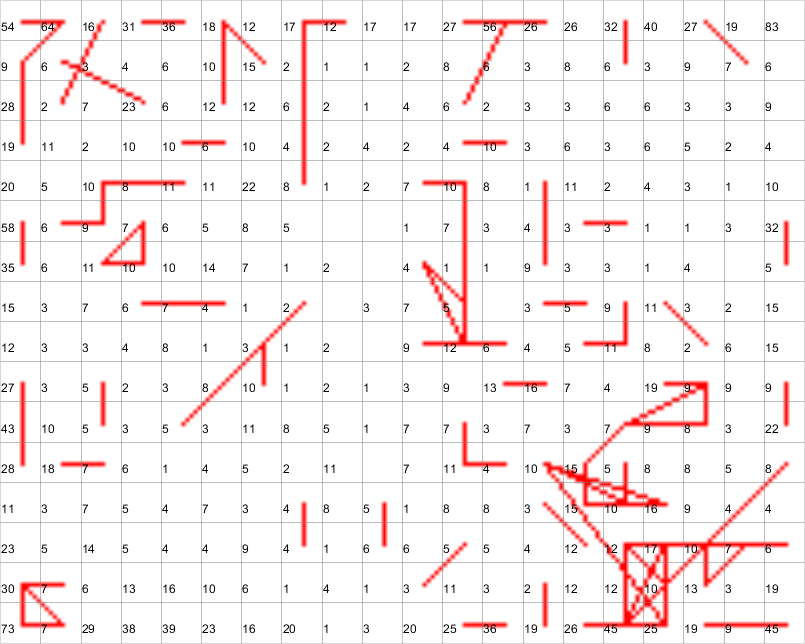
\includegraphics[width=\linewidth]{img/wine-newmid-radius-neighbourhood-graph--r-05-seed-7}
        \caption{$s=7$,$r=0.5$}
        \label{fig:wine-newmid-radius-neighbourhood-graph--r-05-seed-7}
    \end{subfigure}
    \begin{subfigure}[b]{0.30\linewidth}
        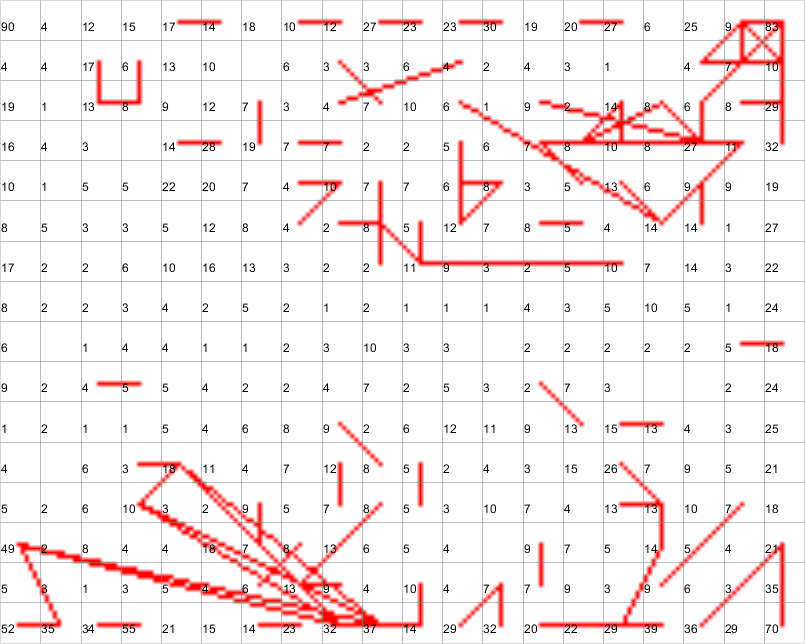
\includegraphics[width=\linewidth]{img/wine-newmid-radius-neighbourhood-graph--r-05-seed-55}
        \caption{$s=55$,$r=0.5$}
        \label{fig:wine-newmid-radius-neighbourhood-graph--r-05-seed-55}
    \end{subfigure}
    \caption{SOM ($20\times16$) Neighbourhood radius with different seed values $s$ and radius $r$}
    \label{fig:wine-newmid-radius-neighbourhood-graph--r-05-seed}
\end{figure}

\begin{figure}
\centering
    \centering
    \begin{subfigure}[b]{0.30\linewidth}
        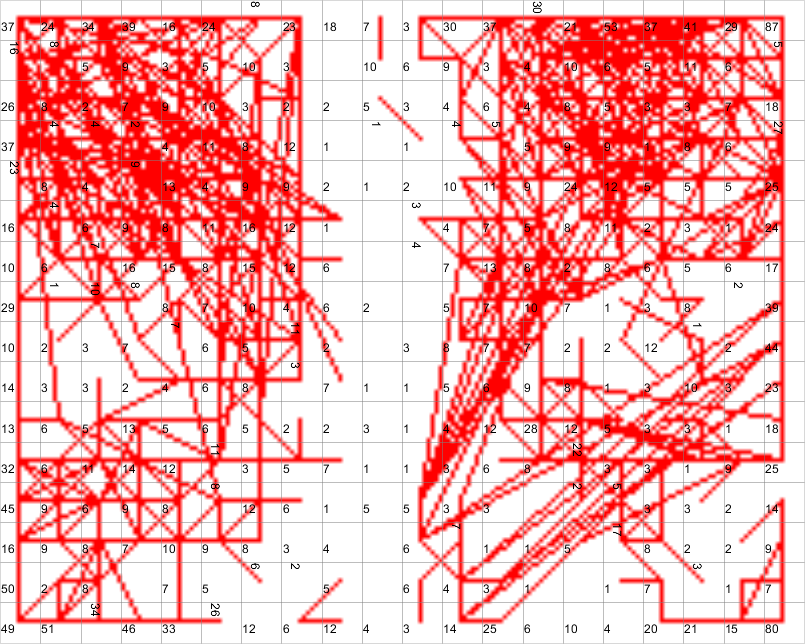
\includegraphics[width=\linewidth]{img/wine-newmid-radius-neighbourhood-graph--r-08-seed-1}
        \caption{$s=1$,$r=0.8$}
        \label{fig:wine-newmid-radius-neighbourhood-graph--r-08-seed-1}
    \end{subfigure}
    \begin{subfigure}[b]{0.30\linewidth}
        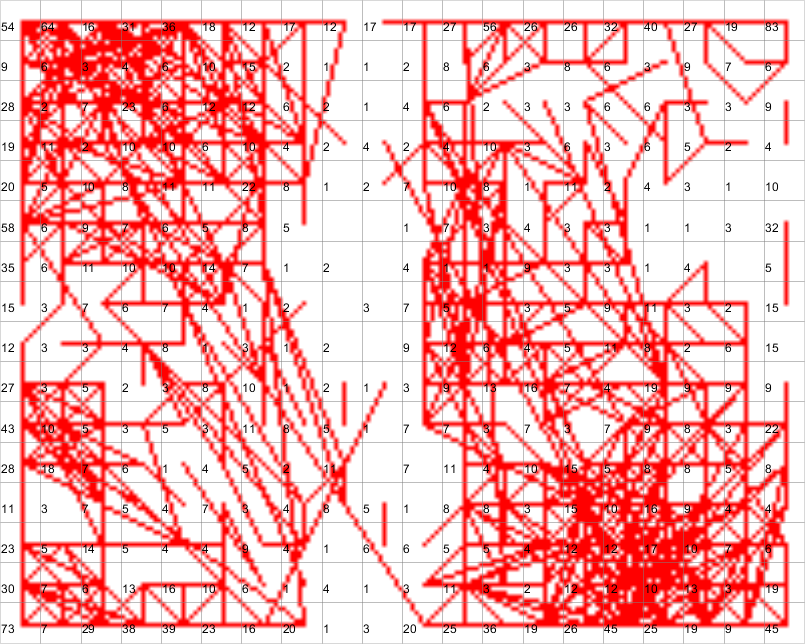
\includegraphics[width=\linewidth]{img/wine-newmid-radius-neighbourhood-graph--r-08-seed-7}
        \caption{$s=7$,$r=0.8$}
        \label{fig:wine-newmid-radius-neighbourhood-graph--r-08-seed-7}
    \end{subfigure}
    \begin{subfigure}[b]{0.30\linewidth}
        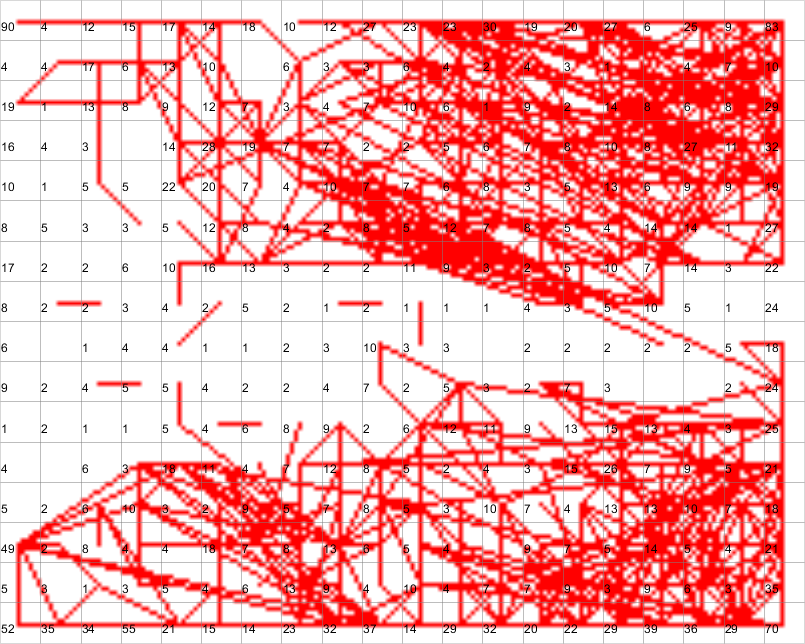
\includegraphics[width=\linewidth]{img/wine-newmid-radius-neighbourhood-graph--r-08-seed-55}
        \caption{$s=55$,$r=0.8$}
        \label{fig:wine-newmid-radius-neighbourhood-graph--r-08-seed-55}
    \end{subfigure}
    \caption{SOM ($20\times16$) Neighbourhood radius with different seed values $s$ and radius $r$}
    \label{fig:wine-newmid-radius-neighbourhood-graph--r-08-seed}
\end{figure}

\begin{figure}
\centering
    \centering
    \begin{subfigure}[b]{0.30\linewidth}
        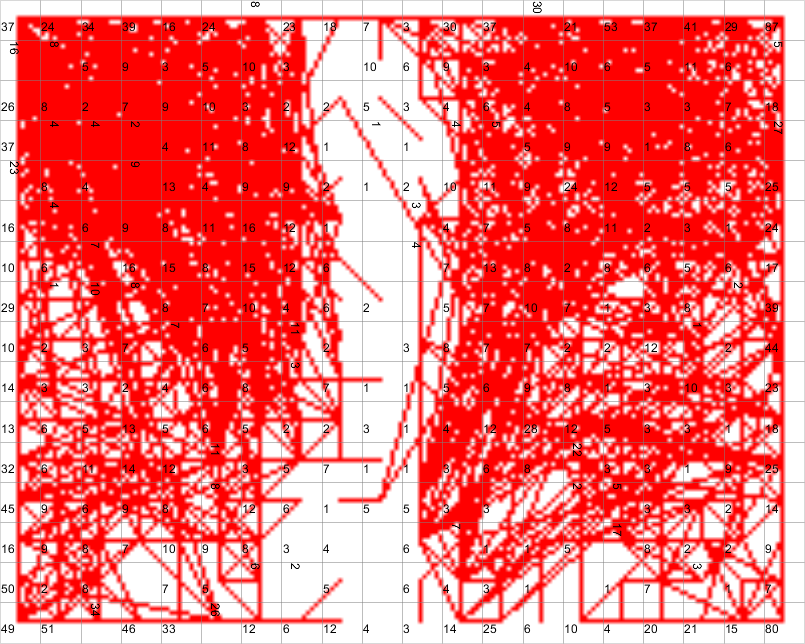
\includegraphics[width=\linewidth]{img/wine-newmid-radius-neighbourhood-graph--r-10-seed-1}
        \caption{$s=1$,$r=1.0$}
        \label{fig:wine-newmid-radius-neighbourhood-graph--r-10-seed-1}
    \end{subfigure}
    \begin{subfigure}[b]{0.30\linewidth}
        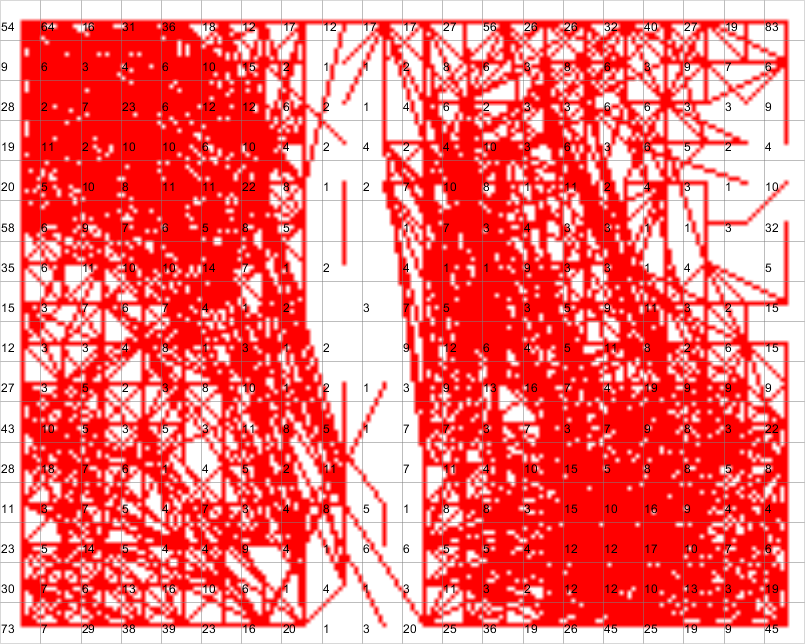
\includegraphics[width=\linewidth]{img/wine-newmid-radius-neighbourhood-graph--r-10-seed-7}
        \caption{$s=7$,$r=1.0$}
        \label{fig:wine-newmid-radius-neighbourhood-graph--r-10-seed-7}
    \end{subfigure}
    \begin{subfigure}[b]{0.30\linewidth}
        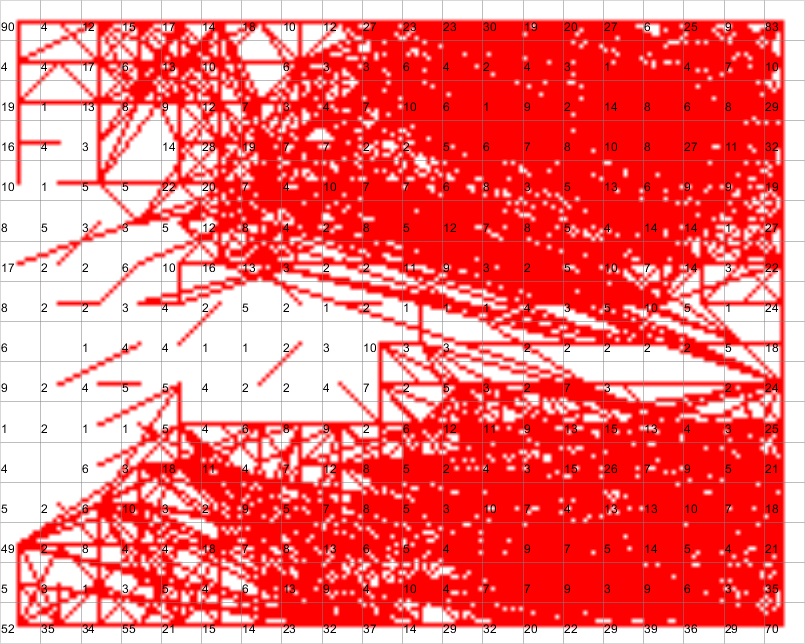
\includegraphics[width=\linewidth]{img/wine-newmid-radius-neighbourhood-graph--r-10-seed-55}
        \caption{$s=55$,$r=1.0$}
        \label{fig:wine-newmid-radius-neighbourhood-graph--r-10-seed-55}
    \end{subfigure}
    \caption{SOM ($20\times16$) Neighbourhood radius with different seed values $s$ and radius $r$}
    \label{fig:wine-newmid-radius-neighbourhood-graph--r-10-seed}
\end{figure}

\begin{figure}
\centering
    \centering
    \begin{subfigure}[b]{0.30\linewidth}
        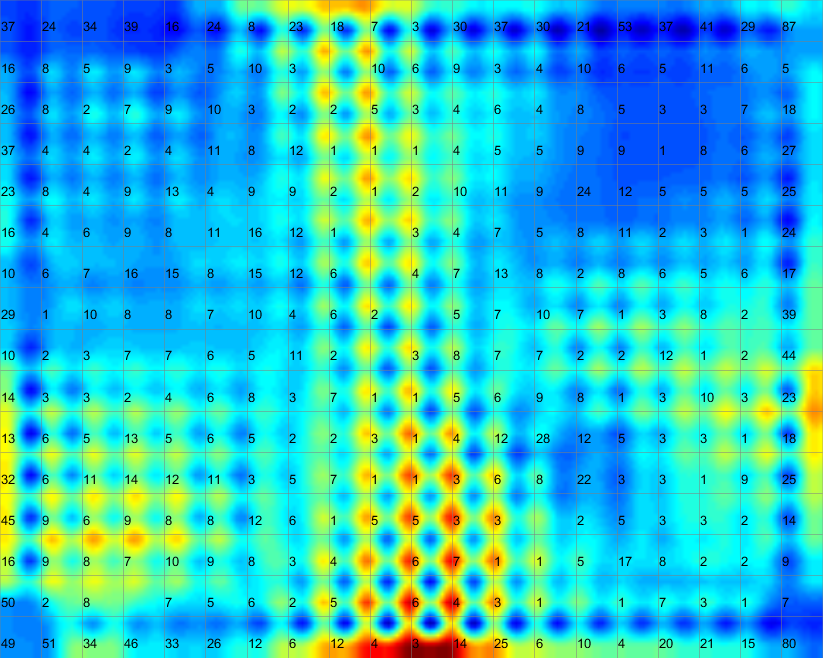
\includegraphics[width=\linewidth]{img/wine-newmid-u-matrix-seed-1}
        \caption{$s=1$}
        \label{fig:wine-newmid-u-matrix-seed-1}
    \end{subfigure}
    \begin{subfigure}[b]{0.30\linewidth}
        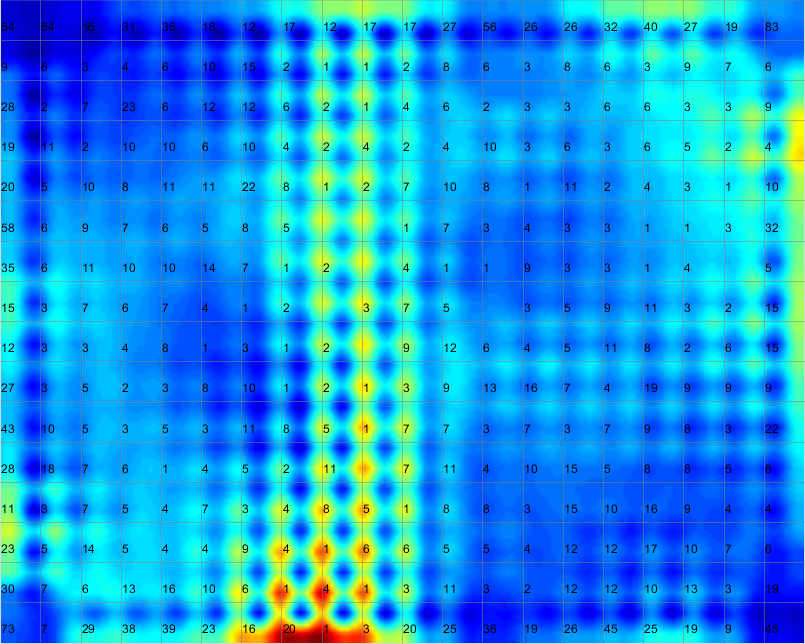
\includegraphics[width=\linewidth]{img/wine-newmid-u-matrix-seed-7}
        \caption{$s=7$}
        \label{fig:wine-newmid-u-matrix-seed-7}
    \end{subfigure}
    \begin{subfigure}[b]{0.30\linewidth}
        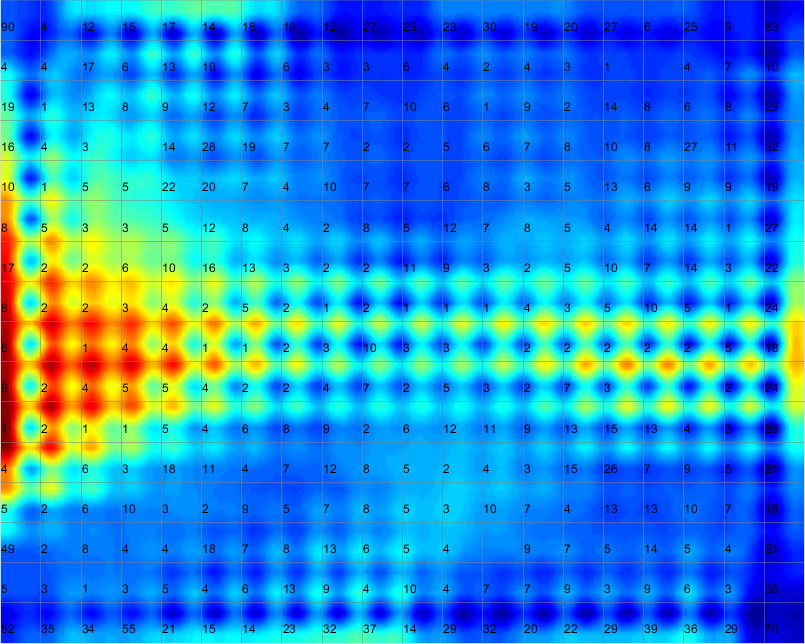
\includegraphics[width=\linewidth]{img/wine-newmid-u-matrix-seed-55}
        \caption{$s=55$}
        \label{fig:wine-newmid-u-matrix-seed-55}
    \end{subfigure}
    \caption{SOM ($20\times16$) U-Matrix with different seed values $s$}
    \label{fig:wine-newmid-u-matrix-seed}
\end{figure}

\section{SOM Normalization. Training not normalized data}

To highlight the difference between a SOM that is trained with erroneous normalized data
we use the settings provided in the Table~\ref{tab:settings}. We found out earlier that a rectangular
SOM is more useful for our data distribution. Thus we now take a look at a $20\times14$ SOM.

As we have discussed earlier, there are attributes that contain outliers.
For those\footnote{Residual Sugar, Chlorides, Free sulfur dioxide, Total sulfur dioxide, Sulphates} we apply min/max scaling. We assume that by using this scaling technique we distort these attributes, which leads to a blur of the two clusters.
For all others we use unit length scaling. As we heard in the lecture this scaling technique
divides by the vector length, thus it makes the attribute vector unit length. This is
not desirable, because we do not want our measurements to look the same. It would
make sense for an attribute like document size, because it is mostly not the document
size that defines the type of content. This is not the case for measurements.

In the following we present the Activity Histogram in Figure~\ref{fig:wine-weird-activity-histogram},
the Smoothed Data Histogram in Figure~\ref{fig:wine-weird-smoothed-data-histogram},
the U-Matrix in Figure~\ref{fig:wine-weird-u-matrix} and
the Nearest Neighbourhood visualization using a radius of 0.1 in Figure~\ref{fig:wine-weird-nearest-neighbour-radius}.

\begin{figure}
\centering
    \centering
    \begin{subfigure}[b]{0.45\linewidth}
        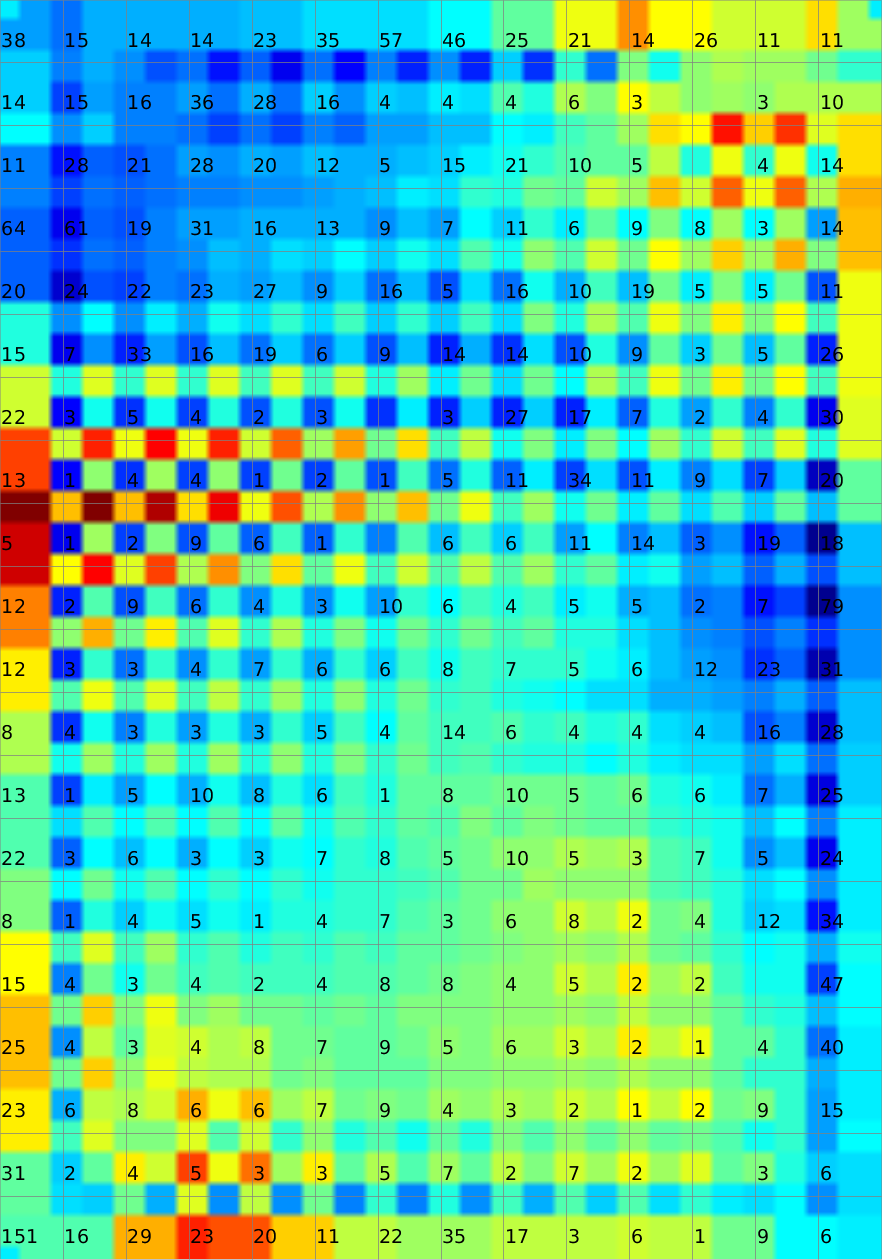
\includegraphics[width=\linewidth]{img/wine-weird-u-matrix}
        \caption{U-Matrix}
        \label{fig:wine-weird-u-matrix}
    \end{subfigure}
    \begin{subfigure}[b]{0.45\linewidth}
        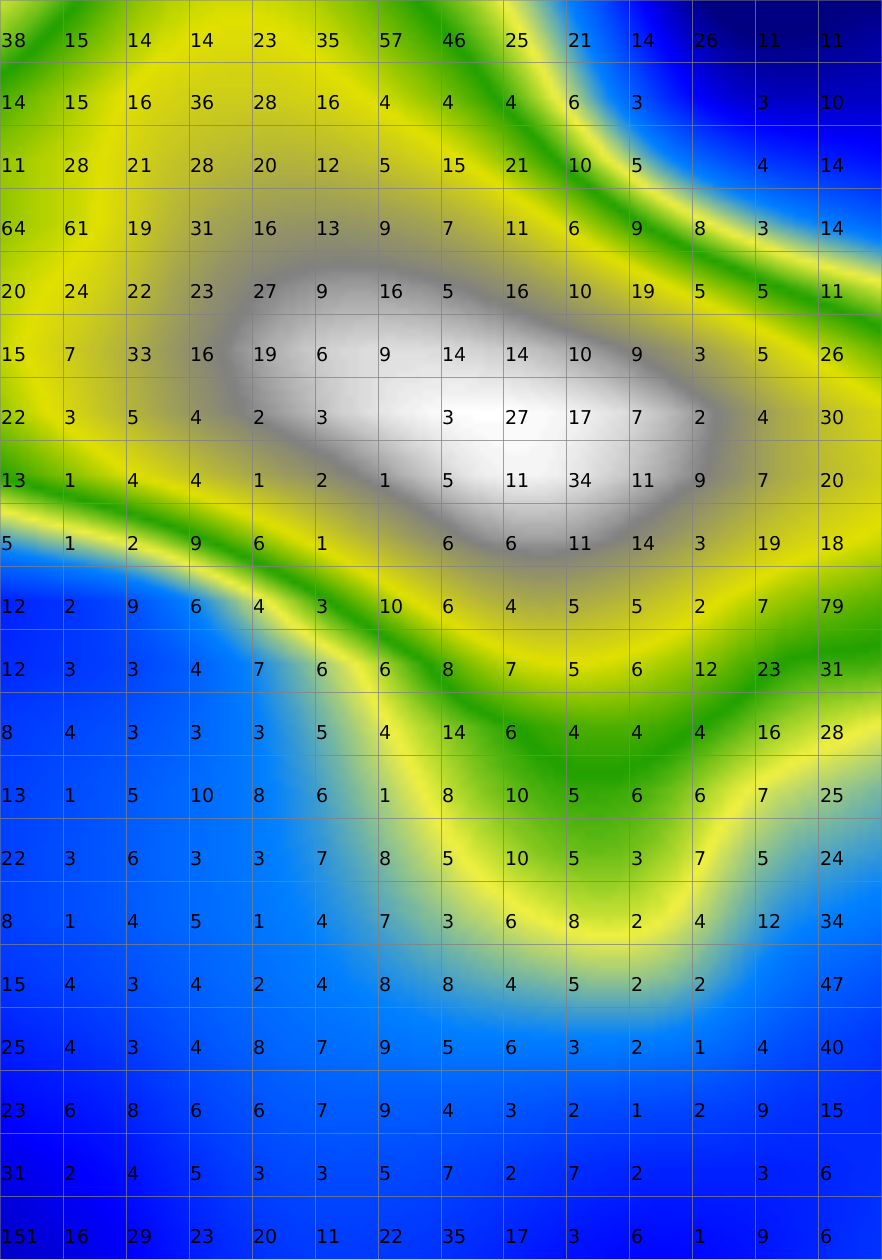
\includegraphics[width=\linewidth]{img/wine-weird-smoothed-data-histogram}
        \caption{SDH smooth factor 149}
        \label{fig:wine-weird-smoothed-data-histogram}
    \end{subfigure}
    \caption{SOM Visualisations of errornous normalized data}
\end{figure}

Comparing the U-Matrix to the previous U Matrices this one has many more mountain
areas. The distinction between clusters and cluster boundaries are not visible.
In the top left there is one coherent valley that is mostly colored blue.
The rest of the map seems not to display any clusters. This is very different, because
earlier we had a clear distinction between two clusters, but here the mountains
take up to more than 80\% of the map.

The Activity Histogram now displays one gradient from the bottom left to the top right.
In the correctly normalized data we do not have such a gradient, and one part of our map
also contained topology violations.

The SDH shows one big area located above in the center. Use a smoothing factor of 149.
When decreasing the smoothing factor the big bulb above the center is still dominant,
but moves into the top left of the map (shown in Figure~\ref{fig:wine-weird-smoothed-data-histogram-series}).
This matches very well the flat vally found in
Figure~\ref{fig:wine-weird-u-matrix}.

The nearest neighbour shows that the units of the SOM are very close to each other. The 
radius is set to 0.1. The picture shows that they are so close together, that
nearly every unit is connected to every other unit.

\begin{figure}
    \centering
    \begin{subfigure}[b]{0.45\linewidth}
        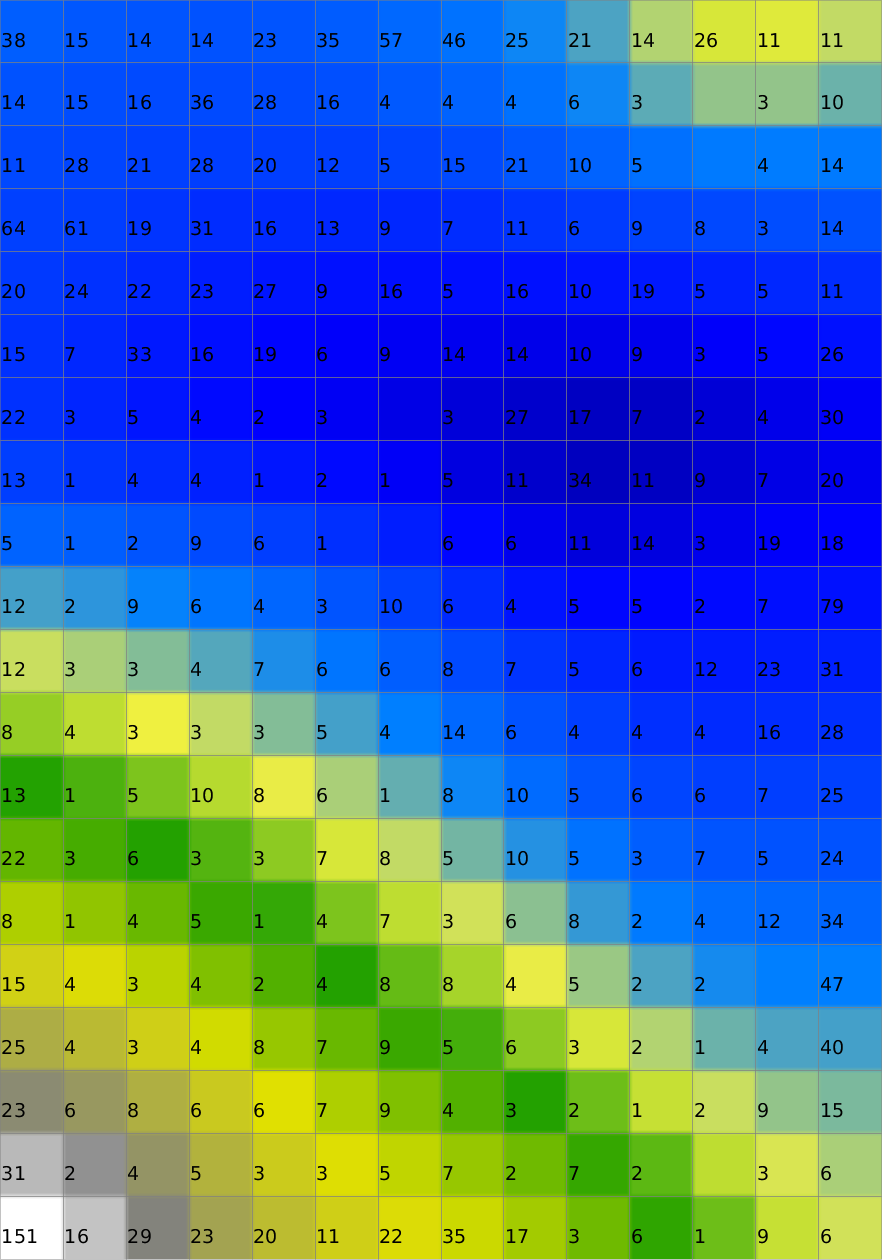
\includegraphics[width=\linewidth]{img/wine-weird-activity-histogram}
        \caption{Activity histogram\\}
        \label{fig:wine-weird-activity-histogram}
    \end{subfigure}
    \begin{subfigure}[b]{0.45\linewidth}
        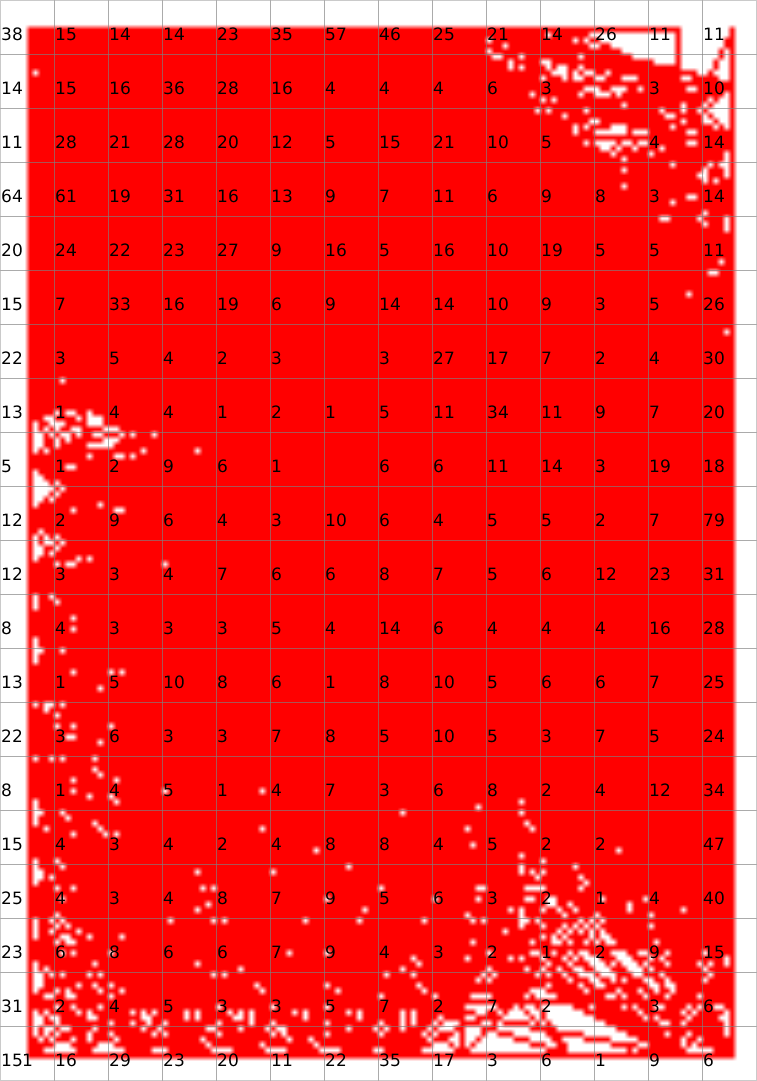
\includegraphics[width=\linewidth]{img/wine-weird-nearest-neighbour-radius}
        \caption{Neighbourhood graph ($r=0.1$)}
        \label{fig:wine-weird-nearest-neighbour-radius}
    \end{subfigure}
    \caption{SOM ($14\times20$) visualisations of errornous normalized data}
\end{figure}

The scaling we applied earlier was quite effective to distort the input data
and map the input data to data that looks very similar. In our opinion
many characteristics of the attributes where lost and we could verify this
in the produced SOM Visualisations.

\begin{figure}
\centering
    \centering
    \begin{subfigure}[b]{0.30\linewidth}
        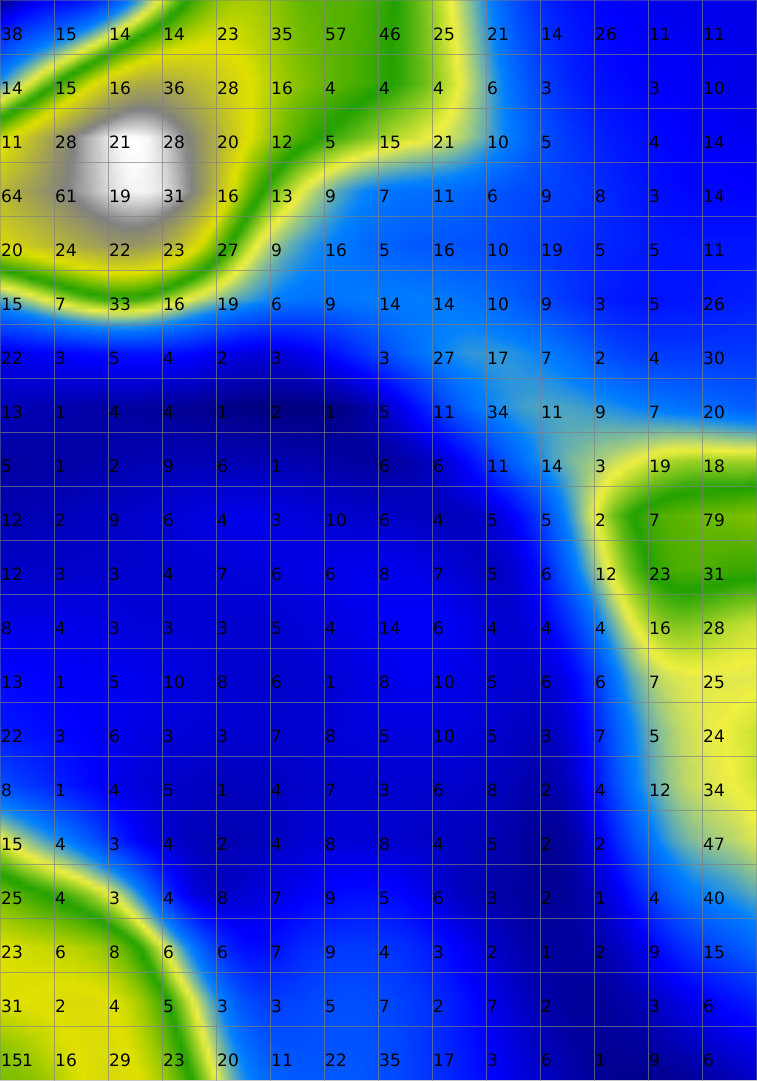
\includegraphics[width=\linewidth]{img/wine-weird-smoothed-data-histogram-20}
        \caption{$f=20$}
    \end{subfigure}
    \begin{subfigure}[b]{0.30\linewidth}
        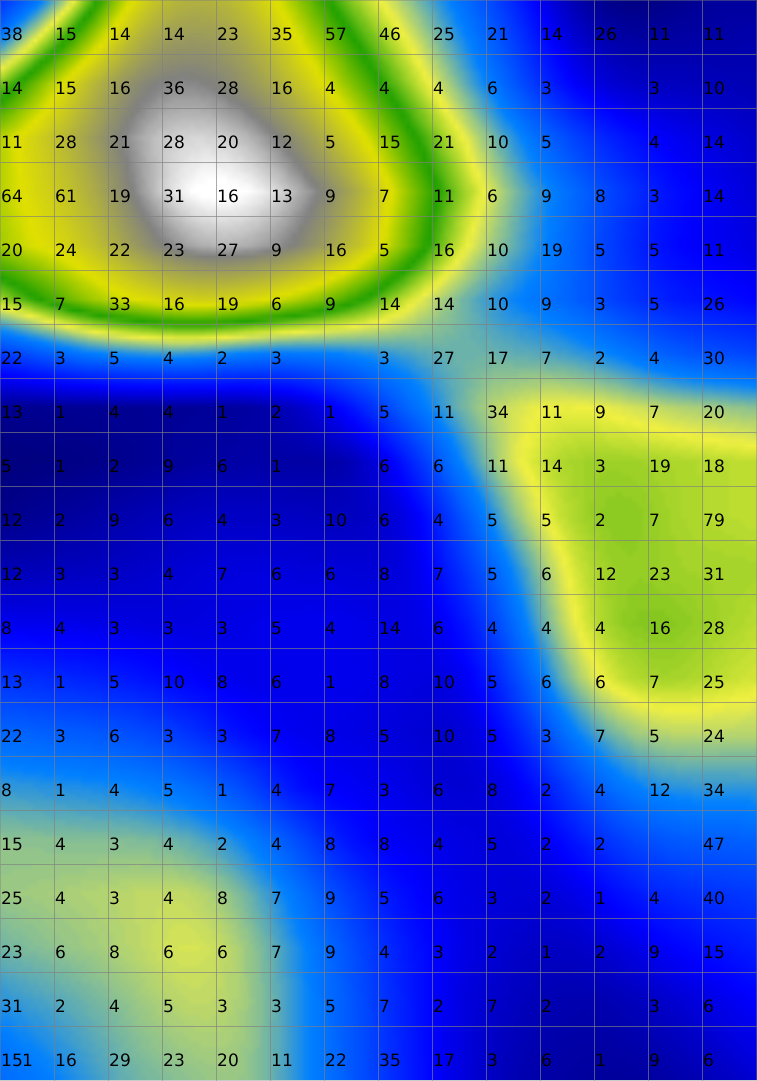
\includegraphics[width=\linewidth]{img/wine-weird-smoothed-data-histogram-50}
        \caption{$f=50$}
    \end{subfigure}
    \begin{subfigure}[b]{0.30\linewidth}
        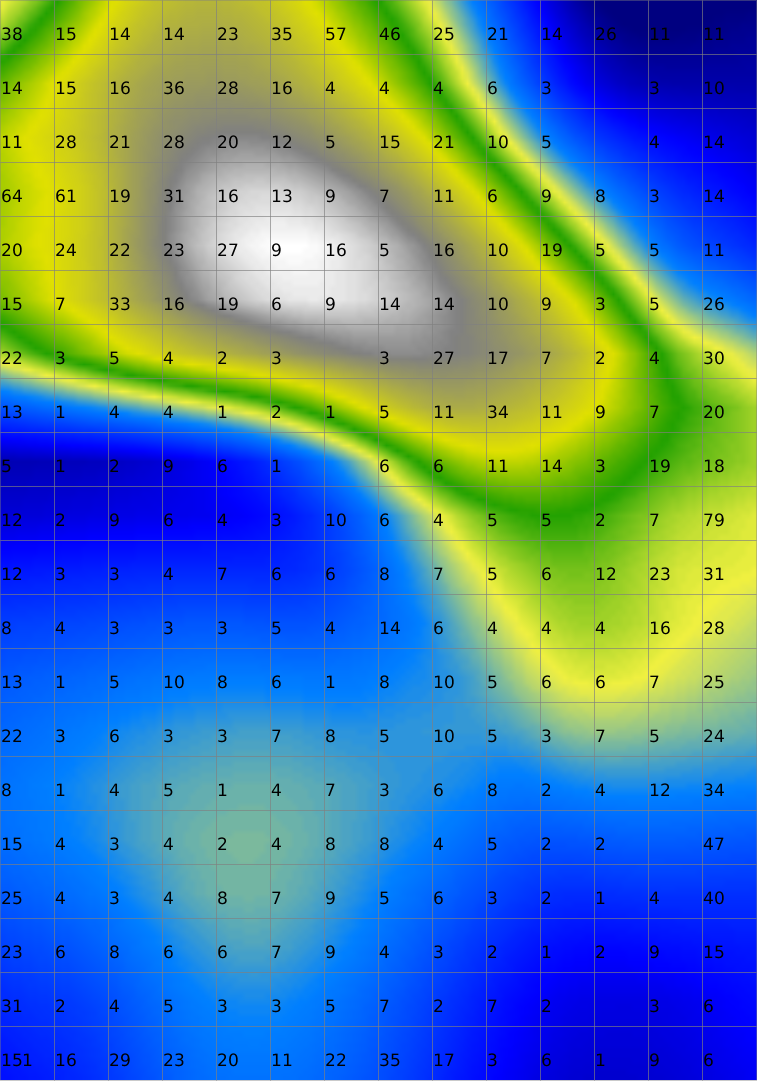
\includegraphics[width=\linewidth]{img/wine-weird-smoothed-data-histogram-100}
        \caption{$f=100$}
    \end{subfigure}
    \caption{SOM ($20\times14$) SDH with different smoothing factor $f$}
    \label{fig:wine-weird-smoothed-data-histogram-series}
\end{figure}

\section{Adjusting the neighbourhood radius for training}

In the following section we show how the neighbourhood radius $\sigma$ affects the map topology
and the structures on the map. We use the settings shown in Table~\ref{tab:settings}.
(Neighbourhood Small to Big).

Our assumption is that for very small neighbourhood radius, only the Best Matching Units and their very close neighbouring units will be adjusted according to the input vectors. This behaviour will leave the map scrambled where very similar units that are not affected by the neighbourhood radius will remain far away causing many topology violations. The other extreme, a very big neighbourhood radius for every Best Matching Unit will cover all of the units of the SOM and thus producing a very powerful units on the diagonals which will lead to mapping many data-samples to them.

For the SDH we used a smoothing factor of 100 instead of the default one. Figure~\ref{fig:wine-newmid-smoothed-data-histogram-sigma-1} shows the revealed clusters for very small $sigma$ which are not correctly formed and isolated. The cluster boundaries are not correctly formed and this is visible on the U-Matrix on Figure~\ref{fig:wine-newmid-u-matrix-sigma-1}. Our assumption for many topology violations is confirmed by observing the Activity Histogram on Figure~\ref{fig:wine-newmid-activity-histogram-sigma}(a) which show many mixed units and on the Topographic Error shown on Figure~\ref{fig:wine-newmid-topographic-error-sigma} showing big number of topology violations.

The better adaptation of the SOM is visible for bigger neighbourhood values. For $sigma = 5$ Figure~\ref{fig:wine-newmid-smoothed-data-histogram-sigma-5} forms clusters and Figure~\ref{fig:wine-newmid-u-matrix-sigma-5} shows clearly defined cluster boundaries with coherent regions. A significant decrease of Topology Violations is noticeable on Figure~\ref{fig:wine-newmid-activity-histogram-sigma}(b) and Figure~\ref{fig:wine-newmid-topographic-error-sigma}(b).

Our assumption for big neighbourhood radius values is confirmed by looking at the number of mapped units to the lower-left and upper-right diagonals. Figure~\ref{fig:wine-newmid-topographic-error-sigma} depicts that the diagonals contain 66/99 mapped units compared to the 44/17 with the diagonals from the SOM with $sigma=5$. Figure~\ref{fig:wine-newmid-smoothed-data-histogram-sigma-15} shows a definition of the main clusters and the cluster boundaries are identified by the U-Matrix. This visualization shows the right cluster boundaries but the regions are not very coherent which is consequence caused by the big neighbourhood radius.


\begin{figure}
\centering
    \centering
    \begin{subfigure}[b]{0.30\linewidth}
        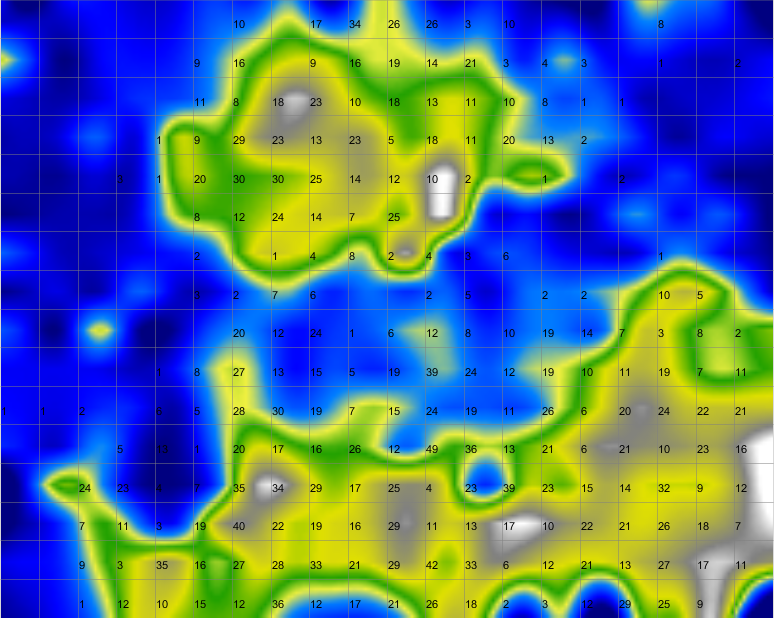
\includegraphics[width=\linewidth]{img/wine-newmid-smoothed-data-histogram-sigma-1}
        \caption{$\sigma=1$}
        \label{fig:wine-newmid-smoothed-data-histogram-sigma-1}
    \end{subfigure}
    \begin{subfigure}[b]{0.30\linewidth}
        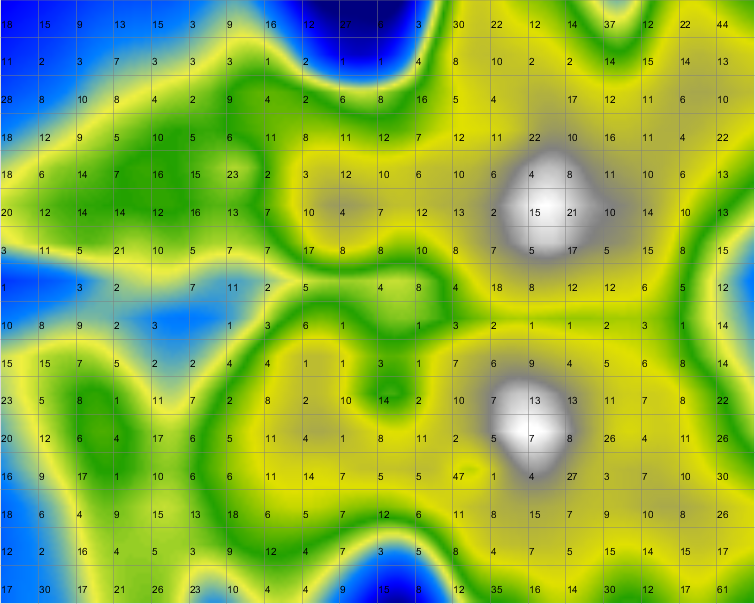
\includegraphics[width=\linewidth]{img/wine-newmid-smoothed-data-histogram-sigma-5}
        \caption{$\sigma=5$}
        \label{fig:wine-newmid-smoothed-data-histogram-sigma-5}
    \end{subfigure}
    \begin{subfigure}[b]{0.30\linewidth}
        \includegraphics[width=\linewidth]{img/wine-newmid-smoothed-data-histogram-sigma-15}
        \caption{$\sigma=15$}
        \label{fig:wine-newmid-smoothed-data-histogram-sigma-15}
    \end{subfigure}
    \caption{SOM ($20\times16$) SDH with different neighbour hood radius$f$}
    \label{fig:wine-newmid-smoothed-data-histogram-sigma}
\end{figure}

\begin{figure}
\centering
    \centering
    \begin{subfigure}[b]{0.30\linewidth}
        \includegraphics[width=\linewidth]{img/wine-newmid-topographic-error-sigma-1}
        \caption{$\sigma=1$}
        \label{fig:wine-newmid-topographic-error-sigma-1}
    \end{subfigure}
    \begin{subfigure}[b]{0.30\linewidth}
        \includegraphics[width=\linewidth]{img/wine-newmid-topographic-error-sigma-5}
        \caption{$\sigma=5$}
        \label{fig:wine-newmid-topographic-error-sigma-5}
    \end{subfigure}
    \begin{subfigure}[b]{0.30\linewidth}
        \includegraphics[width=\linewidth]{img/wine-newmid-topographic-error-sigma-15}
        \caption{$\sigma=15$}
        \label{fig:wine-newmid-topographic-error-sigma-15}
    \end{subfigure}
    \caption{SOM ($20\times16$) Topographic error with different neighbour hood radius$f$}
    \label{fig:wine-newmid-topographic-error-sigma}
\end{figure}

\begin{figure}
\centering
    \centering
    \begin{subfigure}[b]{0.30\linewidth}
        \includegraphics[width=\linewidth]{img/wine-newmid-activity-histogram-sigma-1}
        \caption{$\sigma=1$}
        \label{fig:wine-newmid-activity-histogram-sigma-1}
    \end{subfigure}
    \begin{subfigure}[b]{0.30\linewidth}
        \includegraphics[width=\linewidth]{img/wine-newmid-activity-histogram-sigma-5}
        \caption{$\sigma=5$}
        \label{fig:wine-newmid-activity-histogram-sigma-5}
    \end{subfigure}
    \begin{subfigure}[b]{0.30\linewidth}
        \includegraphics[width=\linewidth]{img/wine-newmid-activity-histogram-sigma-15}
        \caption{$\sigma=15$}
        \label{fig:wine-newmid-activity-histogram-sigma-15}
    \end{subfigure}
    \caption{SOM ($20\times16$) Activity Histograms with different neighbour hood radius$f$}
    \label{fig:wine-newmid-activity-histogram-sigma}
\end{figure}

\begin{figure}
\centering
    \centering
    \begin{subfigure}[b]{0.30\linewidth}
        \includegraphics[width=\linewidth]{img/wine-newmid-u-matrix-sigma-1}
        \caption{$\sigma=1$}
        \label{fig:wine-newmid-u-matrix-sigma-1}
    \end{subfigure}
    \begin{subfigure}[b]{0.30\linewidth}
        \includegraphics[width=\linewidth]{img/wine-newmid-u-matrix-sigma-5}
        \caption{$\sigma=5$}
        \label{fig:wine-newmid-u-matrix-sigma-5}
    \end{subfigure}
    \begin{subfigure}[b]{0.30\linewidth}
        \includegraphics[width=\linewidth]{img/wine-newmid-u-matrix-sigma-15}
        \caption{$\sigma=15$}
        \label{fig:wine-newmid-u-matrix-sigma-15}
    \end{subfigure}
    \caption{SOM ($20\times16$) U-Matrix with different neighbour hood radius$f$}
    \label{fig:wine-newmid-u-matrix-sigma}
\end{figure}

\section{SOM varying learning rate}

In this section we will vary $\alpha$.  Our different settings are displayed in the Table~\ref{tab:settings} (Alpha 0.01, ...).

By looking at the weight vector adjustment equation
\[
    m_i(t+1) = m_i(t) + \alpha(t) * h_{ci}(t) * [x(t) - m_i(t)]
\]
our assumption is that for a small learning rate $\alpha$ the learning component has a very small
influence on adjusting the weight vector towards the input vector.
The problem the might arise is that a small radius will leave the SOM unwrapped.

A very big learning rate on the other hand will force the weight vector to perform a big initial adjustments towards the chosen input vector.
The initial learning step is very powerful, some of the units could be initially moved to
a more distant location in the data space. At later point in time (with decreasing learning rate and neighbourhood radius) the algorithm
will not be powerful enough to pull them to the ``optimal'' location. We think that a big radius should in some cases contain slightly more topology violations.

The Activity histogram in Figure~\ref{fig:wine-20x16-activity-histogram-alpha} shows that a small $\alpha$ radius did not unwrap the map and contains
a lot of topology violations. Figure~\ref{fig:wine-20x16-neighbourhood-graph-r-06-alpha} and Figure~\ref{fig:wine-20x16-quantization-error-alpha} also confirm that the map was unable to unfold.
A small learning rate was unable to separate clusters. This can be seen in Figure~\ref{fig:wine-20x16-u-matrix-alpha}
and
\ref{fig:wine-20x16-smoothed-data-histogram-alpha-f-50}
\ref{fig:wine-20x16-smoothed-data-histogram-alpha-f-100}
\ref{fig:wine-20x16-smoothed-data-histogram-alpha-f-149}
where the cluster boundaries are not visible.

Be increasing the learning rate (greater than 0.45) the difference in almost all of the visualisations in so not so evident.
As an example in Figure~\ref{fig:wine-20x16-activity-histogram-alpha} the revealed clusters do not differ so much. For all of 
them in the Figures
\ref{fig:wine-20x16-smoothed-data-histogram-alpha-f-50}
\ref{fig:wine-20x16-smoothed-data-histogram-alpha-f-100}
the cluster boundaries can be determined. By looking at the U-Matrix the cluster boundaries in Figure~\ref{fig:wine-20x16-u-matrix-alpha}
using a big learning rate (0.99) the visualisations shows more coherent regions.

We mentioned earlier that a big learning rate might increase topology violations.
By looking at Figure~\ref{fig:wine-20x16-neighbourhood-graph-r-06-alpha} we believe that our assumption for
a very big learning rate is visible. Compared to Figure~\ref{fig:wine-20x16-neighbourhood-graph-r-06-alpha-0,7},
\ref{fig:wine-20x16-neighbourhood-graph-r-06-alpha-0,99} displays some long red lines that are not contained in the former.
Still the effect of a high learning rate seems not to hinder the map to unwrap correctly, but a small rate obviously does.

\begin{figure}
\centering
    \centering
    \begin{subfigure}[b]{0.24\linewidth}
        \includegraphics[width=\linewidth]{img/wine-20x16-activity-histogram-alpha-0,01}
        \caption{$\alpha=0.01$}
        \label{fig:wine-20x16-activity-histogram-alpha-0,01}
    \end{subfigure}
    \begin{subfigure}[b]{0.24\linewidth}
        \includegraphics[width=\linewidth]{img/wine-20x16-activity-histogram-alpha-0,45}
        \caption{$\alpha=0.45$}
        \label{fig:wine-20x16-activity-histogram-alpha-0,45}
    \end{subfigure}
    \begin{subfigure}[b]{0.24\linewidth}
        \includegraphics[width=\linewidth]{img/wine-20x16-activity-histogram-alpha-0,7}
        \caption{$\alpha=0.7$}
        \label{fig:wine-20x16-activity-histogram-alpha-0,7}
    \end{subfigure}
    \begin{subfigure}[b]{0.24\linewidth}
        \includegraphics[width=\linewidth]{img/wine-20x16-activity-histogram-alpha-0,99}
        \caption{$\alpha=0.99$}
        \label{fig:wine-20x16-activity-histogram-alpha-0,99}
    \end{subfigure}
    \caption{SOM ($20\times16$) Activity histogram (varied $\alpha$)}
    \label{fig:wine-20x16-activity-histogram-alpha}
\end{figure}

\begin{figure}
\centering
    \centering
    \begin{subfigure}[b]{0.24\linewidth}
        \includegraphics[width=\linewidth]{img/wine-20x16-smoothed-data-histogram-alpha-0,01-f-50}
        \caption{$\alpha=0.01$}
        \label{fig:wine-20x16-smoothed-data-histogram-alpha-0,01-f-50}
    \end{subfigure}
    \begin{subfigure}[b]{0.24\linewidth}
        \includegraphics[width=\linewidth]{img/wine-20x16-smoothed-data-histogram-alpha-0,45-f-50}
        \caption{$\alpha=0.45$}
        \label{fig:wine-20x16-smoothed-data-histogram-alpha-0,45-f-50}
    \end{subfigure}
    \begin{subfigure}[b]{0.24\linewidth}
        \includegraphics[width=\linewidth]{img/wine-20x16-smoothed-data-histogram-alpha-0,7-f-50}
        \caption{$\alpha=0.7$}
        \label{fig:wine-20x16-smoothed-data-histogram-alpha-0,7-f-50}
    \end{subfigure}
    \begin{subfigure}[b]{0.24\linewidth}
        \includegraphics[width=\linewidth]{img/wine-20x16-smoothed-data-histogram-alpha-0,99-f-50}
        \caption{$\alpha=0.99$}
        \label{fig:wine-20x16-smoothed-data-histogram-alpha-0,99-f-50}
    \end{subfigure}
    \caption{SOM ($20\times16$) SDH (varied $\alpha$), smooth factor 50}
    \label{fig:wine-20x16-smoothed-data-histogram-alpha-f-50}
\end{figure}

\begin{figure}
\centering
    \centering
    \begin{subfigure}[b]{0.24\linewidth}
        \includegraphics[width=\linewidth]{img/wine-20x16-smoothed-data-histogram-alpha-0,01-f-100}
        \caption{$\alpha=0.01$}
        \label{fig:wine-20x16-smoothed-data-histogram-alpha-0,01-f-100}
    \end{subfigure}
    \begin{subfigure}[b]{0.24\linewidth}
        \includegraphics[width=\linewidth]{img/wine-20x16-smoothed-data-histogram-alpha-0,45-f-100}
        \caption{$\alpha=0.45$}
        \label{fig:wine-20x16-smoothed-data-histogram-alpha-0,45-f-100}
    \end{subfigure}
    \begin{subfigure}[b]{0.24\linewidth}
        \includegraphics[width=\linewidth]{img/wine-20x16-smoothed-data-histogram-alpha-0,7-f-100}
        \caption{$\alpha=0.7$}
        \label{fig:wine-20x16-smoothed-data-histogram-alpha-0,7-f-100}
    \end{subfigure}
    \begin{subfigure}[b]{0.24\linewidth}
        \includegraphics[width=\linewidth]{img/wine-20x16-smoothed-data-histogram-alpha-0,99-f-100}
        \caption{$\alpha=0.99$}
        \label{fig:wine-20x16-smoothed-data-histogram-alpha-0,99-f-100}
    \end{subfigure}
    \caption{SOM ($20\times16$) SDH (varied $\alpha$), smooth factor 100}
    \label{fig:wine-20x16-smoothed-data-histogram-alpha-f-100}
\end{figure}

\begin{figure}
\centering
    \centering
    \begin{subfigure}[b]{0.24\linewidth}
        \includegraphics[width=\linewidth]{img/wine-20x16-smoothed-data-histogram-alpha-0,01-f-149}
        \caption{$\alpha=0.01$}
        \label{fig:wine-20x16-smoothed-data-histogram-alpha-0,01-f-149}
    \end{subfigure}
    \begin{subfigure}[b]{0.24\linewidth}
        \includegraphics[width=\linewidth]{img/wine-20x16-smoothed-data-histogram-alpha-0,45-f-149}
        \caption{$\alpha=0.45$}
        \label{fig:wine-20x16-smoothed-data-histogram-alpha-0,45-f-149}
    \end{subfigure}
    \begin{subfigure}[b]{0.24\linewidth}
        \includegraphics[width=\linewidth]{img/wine-20x16-smoothed-data-histogram-alpha-0,7-f-149}
        \caption{$\alpha=0.7$}
        \label{fig:wine-20x16-smoothed-data-histogram-alpha-0,7-f-149}
    \end{subfigure}
    \begin{subfigure}[b]{0.24\linewidth}
        \includegraphics[width=\linewidth]{img/wine-20x16-smoothed-data-histogram-alpha-0,99-f-149}
        \caption{$\alpha=0.99$}
        \label{fig:wine-20x16-smoothed-data-histogram-alpha-0,99-f-149}
    \end{subfigure}
    \caption{SOM ($20\times16$) SDH (varied $\alpha$), smooth factor 149}
    \label{fig:wine-20x16-smoothed-data-histogram-alpha-f-149}
\end{figure}

\begin{figure}
\centering
    \centering
    \begin{subfigure}[b]{0.24\linewidth}
        \includegraphics[width=\linewidth]{img/wine-20x16-neighbourhood-graph-r-06-alpha-0,01}
        \caption{$\alpha=0.01$}
        \label{fig:wine-20x16-neighbourhood-graph-r-06-alpha-0,01}
    \end{subfigure}
    \begin{subfigure}[b]{0.24\linewidth}
        \includegraphics[width=\linewidth]{img/wine-20x16-neighbourhood-graph-r-06-alpha-0,45}
        \caption{$\alpha=0.45$}
        \label{fig:wine-20x16-neighbourhood-graph-r-06-alpha-0,45}
    \end{subfigure}
    \begin{subfigure}[b]{0.24\linewidth}
        \includegraphics[width=\linewidth]{img/wine-20x16-neighbourhood-graph-r-06-alpha-0,7}
        \caption{$\alpha=0.7$}
        \label{fig:wine-20x16-neighbourhood-graph-r-06-alpha-0,7}
    \end{subfigure}
    \begin{subfigure}[b]{0.24\linewidth}
        \includegraphics[width=\linewidth]{img/wine-20x16-neighbourhood-graph-r-06-alpha-0,99}
        \caption{$\alpha=0.99$}
        \label{fig:wine-20x16-neighbourhood-graph-r-06-alpha-0,99}
    \end{subfigure}
    \caption{SOM ($20\times16$) Neighbourhood radius $r=0.6$ (varied $\alpha$)}
    \label{fig:wine-20x16-neighbourhood-graph-r-06-alpha}
\end{figure}

\begin{figure}
\centering
    \centering
    \begin{subfigure}[b]{0.24\linewidth}
        \includegraphics[width=\linewidth]{img/wine-20x16-quantization-error-alpha-0,01}
        \caption{$\alpha=0.01$}
        \label{fig:wine-20x16-quantization-error-alpha-0,01}
    \end{subfigure}
    \begin{subfigure}[b]{0.24\linewidth}
        \includegraphics[width=\linewidth]{img/wine-20x16-quantization-error-alpha-0,45}
        \caption{$\alpha=0.45$}
        \label{fig:wine-20x16-quantization-error-alpha-0,45}
    \end{subfigure}
    \begin{subfigure}[b]{0.24\linewidth}
        \includegraphics[width=\linewidth]{img/wine-20x16-quantization-error-alpha-0,7}
        \caption{$\alpha=0.7$}
        \label{fig:wine-20x16-quantization-error-alpha-0,7}
    \end{subfigure}
    \begin{subfigure}[b]{0.24\linewidth}
        \includegraphics[width=\linewidth]{img/wine-20x16-quantization-error-alpha-0,99}
        \caption{$\alpha=0.99$}
        \label{fig:wine-20x16-quantization-error-alpha-0,99}
    \end{subfigure}
    \caption{SOM ($20\times16$) Quantization error (varied $\alpha$)}
    \label{fig:wine-20x16-quantization-error-alpha}
\end{figure}

\begin{figure}
\centering
    \centering
    \begin{subfigure}[b]{0.24\linewidth}
        \includegraphics[width=\linewidth]{img/wine-20x16-u-matrix-alpha-0,01}
        \caption{$\alpha=0.01$}
        \label{fig:wine-20x16-u-matrix-alpha-0,01}
    \end{subfigure}
    \begin{subfigure}[b]{0.24\linewidth}
        \includegraphics[width=\linewidth]{img/wine-20x16-u-matrix-alpha-0,45}
        \caption{$\alpha=0.45$}
        \label{fig:wine-20x16-u-matrix-alpha-0,45}
    \end{subfigure}
    \begin{subfigure}[b]{0.24\linewidth}
        \includegraphics[width=\linewidth]{img/wine-20x16-u-matrix-alpha-0,7}
        \caption{$\alpha=0.7$}
        \label{fig:wine-20x16-u-matrix-alpha-0,7}
    \end{subfigure}
    \begin{subfigure}[b]{0.24\linewidth}
        \includegraphics[width=\linewidth]{img/wine-20x16-u-matrix-alpha-0,99}
        \caption{$\alpha=0.99$}
        \label{fig:wine-20x16-u-matrix-alpha-0,99}
    \end{subfigure}
    \caption{SOM ($20\times16$) U-Matrix (varied $\alpha$)}
    \label{fig:wine-20x16-u-matrix-alpha}
\end{figure}

\section{SOM varying iterations}

In this section we will vary the amount of iterations. We tried to train below 5 iterations but the tool was not able to output the trained SOM.
Our different settings are displayed in the Table~\ref{tab:settings}.

By looking at the quantisation error in Figure~\ref{fig:wine-newmid-quantization-error-i-10}, 
we see that there are many interpolating units. This means there are far to few iterations to
distribute the map unit to the data. Figure~\ref{fig:wine-newmid-quantization-error-i-50} shows
a similar picture. On the right side there are less interpolating unit. As the iterations increased
the map unfolded more into right direction.\footnote{We verified this by looking at fuzzy coloring, but did not include the picture}.
For more than 500 iterations as shown in Figure~\ref{fig:wine-newmid-quantization-error-i-500} the map unfolded throughout the data space.
Even by looking at Figure~\ref{fig:wine-newmid-quantization-error-i-10000} the map shows very little change in the middle which
is caused by the fine tuning of the map.

The U-Matrices reveal more information about the cluster boundaries the more iterations it runs.
In Figure~\ref{fig:wine-newmid-u-matrix-i-10} and 
Figure~\ref{fig:wine-newmid-u-matrix-i-50} the cluster boundaries either not formed or started to form. The
former has a huge valley in the top right. This might trick the viewer and let him assume that this is a cluster.
In Figure~\ref{fig:wine-newmid-u-matrix-i-500} the cluster boundaries are formed but not yet complete.

The left and right clusters are separated by a vertical mount region, but each of them contain a
mount region on their own. In Figure~\ref{fig:wine-newmid-u-matrix-i-10000} the fine tuning phase cleared these mountains and
left the cluster boundaries in the middle.

We further analyse the cluster using the SDH visualization. In Figure~\ref{fig:wine-newmid-smoothed-data-histogram-i-10} the
clusters seem scrambled. The reason for this is the low number of iterations.
In Figure~\ref{fig:wine-newmid-smoothed-data-histogram-i-50} a new cluster arises to the right. We mentioned earlier that 
with 50 iterations the map unfolded into the right direction. By further increasing the number of iterations
(shown in Figure~\ref{fig:wine-newmid-smoothed-data-histogram-i-500}) the right cluster starts to divide whereas the left region
a new cluster is formed. At this point the cluster boundaries are clearly formed. In the fine tuning phase
shown in Figure~\ref{fig:wine-newmid-smoothed-data-histogram-i-10000} subcluster emerged. We believe that these might point to different
qualities.

To find topology violations we use both the activity histogram and the topographic error (k=8).
Figure~\ref{fig:wine-newmid-topographic-error-i-10} and~\ref{fig:wine-newmid-topographic-error-i-50} they show many errors.
This is expected because the map did not have time to unfold. A very interesting observation can be
visualized in Figure~\ref{fig:wine-newmid-topographic-error-i-500} and~\ref{fig:wine-newmid-topographic-error-i-10000}.
Not many errors arise in the first, but significantly more in the latter. After 10.000 iterations is very well adjusted to
the dataspace.

Figure~\ref{fig:wine-newmid-activity-histogram-i-10} and~\ref{fig:wine-newmid-activity-histogram-i-50} show the activity
histogram with 10 and 50 iterations respectivley. They show topology violations (scattered colors) in both of them.
By comparing Figure~\ref{fig:wine-newmid-activity-histogram-i-500} and~\ref{fig:wine-newmid-activity-histogram-i-10000} 
we see that there is only one big difference in the top left area.


\begin{figure}
\centering
    \centering
    \begin{subfigure}[b]{0.24\linewidth}
        \includegraphics[width=\linewidth]{img/wine-newmid-quantization-error-i-10}
        \caption{$i=10$}
        \label{fig:wine-newmid-quantization-error-i-10}
    \end{subfigure}
    \begin{subfigure}[b]{0.24\linewidth}
        \includegraphics[width=\linewidth]{img/wine-newmid-quantization-error-i-50}
        \caption{$i=50$}
        \label{fig:wine-newmid-quantization-error-i-50}
    \end{subfigure}
    \begin{subfigure}[b]{0.24\linewidth}
        \includegraphics[width=\linewidth]{img/wine-newmid-quantization-error-i-500}
        \caption{$i=500$}
        \label{fig:wine-newmid-quantization-error-i-500}
    \end{subfigure}
    \begin{subfigure}[b]{0.24\linewidth}
        \includegraphics[width=\linewidth]{img/wine-newmid-quantization-error-i-10000}
        \caption{$i=10000$}
        \label{fig:wine-newmid-quantization-error-i-10000}
    \end{subfigure}
    \caption{SOM ($20\times16$) Quantization error (varying iterations $i$)}
    \label{fig:wine-newmid-quantization-error-i}
\end{figure}


\begin{figure}
\centering
    \centering
    \begin{subfigure}[b]{0.24\linewidth}
        \includegraphics[width=\linewidth]{img/wine-newmid-u-matrix-i-10}
        \caption{$i=10$}
        \label{fig:wine-newmid-u-matrix-i-10}
    \end{subfigure}
    \begin{subfigure}[b]{0.24\linewidth}
        \includegraphics[width=\linewidth]{img/wine-newmid-u-matrix-i-50}
        \caption{$i=50$}
        \label{fig:wine-newmid-u-matrix-i-50}
    \end{subfigure}
    \begin{subfigure}[b]{0.24\linewidth}
        \includegraphics[width=\linewidth]{img/wine-newmid-u-matrix-i-500}
        \caption{$i=500$}
        \label{fig:wine-newmid-u-matrix-i-500}
    \end{subfigure}
    \begin{subfigure}[b]{0.24\linewidth}
        \includegraphics[width=\linewidth]{img/wine-newmid-u-matrix-i-10000}
        \caption{$i=10000$}
        \label{fig:wine-newmid-u-matrix-i-10000}
    \end{subfigure}
    \caption{SOM ($20\times16$) U-Matrix (varying iterations $i$)}
    \label{fig:wine-newmid-u-matrix-i}
\end{figure}

\begin{figure}
\centering
    \centering
    \begin{subfigure}[b]{0.24\linewidth}
        \includegraphics[width=\linewidth]{img/wine-newmid-smoothed-data-histogram-i-10}
        \caption{$i=10$}
        \label{fig:wine-newmid-smoothed-data-histogram-i-10}
    \end{subfigure}
    \begin{subfigure}[b]{0.24\linewidth}
        \includegraphics[width=\linewidth]{img/wine-newmid-smoothed-data-histogram-i-50}
        \caption{$i=50$}
        \label{fig:wine-newmid-smoothed-data-histogram-i-50}
    \end{subfigure}
    \begin{subfigure}[b]{0.24\linewidth}
        \includegraphics[width=\linewidth]{img/wine-newmid-smoothed-data-histogram-i-500}
        \caption{$i=500$}
        \label{fig:wine-newmid-smoothed-data-histogram-i-500}
    \end{subfigure}
    \begin{subfigure}[b]{0.24\linewidth}
        \includegraphics[width=\linewidth]{img/wine-newmid-smoothed-data-histogram-i-10000}
        \caption{$i=10000$}
        \label{fig:wine-newmid-smoothed-data-histogram-i-10000}
    \end{subfigure}
    \caption{SOM ($20\times16$) SDH (varying iterations $i$)}
    \label{fig:wine-newmid-smoothed-data-histogram-i}
\end{figure}


\begin{figure}
\centering
    \centering
    \begin{subfigure}[b]{0.24\linewidth}
        \includegraphics[width=\linewidth]{img/wine-newmid-topographic-error-i-10}
        \caption{$i=10$}
        \label{fig:wine-newmid-topographic-error-i-10}
    \end{subfigure}
    \begin{subfigure}[b]{0.24\linewidth}
        \includegraphics[width=\linewidth]{img/wine-newmid-topographic-error-i-50}
        \caption{$i=50$}
        \label{fig:wine-newmid-topographic-error-i-50}
    \end{subfigure}
    \begin{subfigure}[b]{0.24\linewidth}
        \includegraphics[width=\linewidth]{img/wine-newmid-topographic-error-i-500}
        \caption{$i=500$}
        \label{fig:wine-newmid-topographic-error-i-500}
    \end{subfigure}
    \begin{subfigure}[b]{0.24\linewidth}
        \includegraphics[width=\linewidth]{img/wine-newmid-topographic-error-i-10000}
        \caption{$i=10000$}
        \label{fig:wine-newmid-topographic-error-i-10000}
    \end{subfigure}
    \caption{SOM ($20\times16$) Topographic error 8 (varying iterations $i$)}
    \label{fig:wine-newmid-topographic-error-i}
\end{figure}

\begin{figure}
\centering
    \centering
    \begin{subfigure}[b]{0.24\linewidth}
        \includegraphics[width=\linewidth]{img/wine-newmid-activity-histogram-i-10}
        \caption{$i=10$}
        \label{fig:wine-newmid-activity-histogram-i-10}
    \end{subfigure}
    \begin{subfigure}[b]{0.24\linewidth}
        \includegraphics[width=\linewidth]{img/wine-newmid-activity-histogram-i-50}
        \caption{$i=50$}
        \label{fig:wine-newmid-activity-histogram-i-50}
    \end{subfigure}
    \begin{subfigure}[b]{0.24\linewidth}
        \includegraphics[width=\linewidth]{img/wine-newmid-activity-histogram-i-500}
        \caption{$i=500$}
        \label{fig:wine-newmid-activity-histogram-i-500}
    \end{subfigure}
    \begin{subfigure}[b]{0.24\linewidth}
        \includegraphics[width=\linewidth]{img/wine-newmid-activity-histogram-i-10000}
        \caption{$i=10000$}
        \label{fig:wine-newmid-activity-histogram-i-10000}
    \end{subfigure}
    \caption{SOM ($20\times16$) Activity histogram (varying iterations $i$)}
    \label{fig:wine-newmid-activity-histogram-i}
\end{figure}

\section{Summary}

We have shown many different visualizations and quality measures for WQ dataset using different
parameter settings. The main structures
we found are the two clusters. Red and white wine. Their separation is quite clear. Half of 
the map is dedicated to white wine and the other is dedicated to red wine.
The two clusters where revealed by SDH and the U-Matrix (e.g. Figure~\ref{fig:wine-mid-u-matrix}).

Considering the density, it is similar in both clusters. Around the cluster boundaries there is
very high density shown by the P-Matrix (e.g. Figure~\ref{fig:wine-mid-p-matrix}). 
The details of the density can be revealed by the neighbour hood radius graph.
It shows high density in the left upper area and high density in the lower right area in
Figure~\ref{fig:wine-newmid-radius-neighbourhood-graph--r-08-seed-7} and Figure~\ref{fig:wine-newmid-radius-neighbourhood-graph--r-10-seed-7}-

Topology violations exist in practically all our trained maps. We think that WQ dataset has
a very complex structure. Especially the red wine cluster probably has a spheric form.
The reson for this the different activity histograms (e.g. Figure~\ref{fig:wine-newmid-activity-histogram-seed-7}) see a blue area surrounded by green ring. The blue area is probably the top of the sphere and
under it the green area of the red wine cluster. In the white wine area on the bottom left
there is also a potential subcluster that outlies the other white wines.

To conclude the structure we would like to show the thematic class map in Figure~\ref{fig:wine-newmid-thermatic-class-map}. The settings are the rectangular mid sized map shown in Table~\ref{tab:settings}.
Here again we see that there are two clusters. Each of them seem to have their subclusters depending
on the quality of the wine. As an example the quality white wine are located in the upper left area of
the map which is a dense region. This shows that the quality white wine are very similar.
This is not the case for red wine as the quality wines are located in the upper right area which is
not that dense.

\subsection{Attributes correlation}
The correlation of the attributes was investigated with Metro Maps. The component planes of the attributes combined in Metro Map with $bin=3$
are displayed in Figure~\ref{fig:wine-newmid-metro-map-bin-3} and with $Bin=6$ are displayed in Figure~\ref{fig:wine-newmid-metro-map-bin-6}.
We immediately notice three main groups of correlated attributes. The first group contains: Alcohol and Density, whereas the second group contains: Fixed Acidity and Residual Sugar. The third group contains all the rest attributes.

A very interesting finding is that the quality white wines contain high alcohol values (Figure~\ref{fig:wine-newmid-thematic-component-plane-alcohol}) compared to the rest of the wines.
Quality Red Wines contain lower alcohol values compared to the white wines, but they contain higher Fixed Acidity (Figure~\ref{fig:wine-newmid-thematic-component-plane-fixed-acidity})
and Citric Acid values (Figure~\ref{fig:wine-newmid-thematic-component-plane-citric-acid}). Average White Wines are high in Sugar shown in Figure~\ref{fig:wine-newmid-thematic-component-plane-sugar} where average Red Wines have very low citric acid.

\begin{figure}
\centering
    \centering
    \begin{subfigure}[b]{0.48\linewidth}
        \includegraphics[width=\linewidth]{img/wine-newmid-thematic-metro-map-bins-3}
        \caption{$Bin=3$}
        \label{fig:wine-newmid-metro-map-bin-3}
    \end{subfigure}
    \begin{subfigure}[b]{0.48\linewidth}
        \includegraphics[width=\linewidth]{img/wine-newmid-thematic-metro-map-bins-6}
        \caption{$Bin=6$}
        \label{fig:wine-newmid-metro-map-bin-6}
    \end{subfigure}
    \begin{subfigure}[b]{0.30\linewidth}
        \includegraphics[width=\linewidth]{img/wine-newmid-thematic-metro-map-legend}
        \caption{Color legend}
    \end{subfigure}
    \caption{SOM ($20\times16$ Rectangular mid sized map in Table~\ref{tab:settings}) Metro Maps and the attribute Legend.}
    \label{fig:wine-newmid-metro-maps}
\end{figure}

\begin{figure}
\centering
    \centering
    \begin{subfigure}[b]{0.48\linewidth}
        \includegraphics[width=\linewidth]{img/wine-newmid-thematic-component-plane-alcohol}
        \caption{Alcohol}
        \label{fig:wine-newmid-thematic-component-plane-alcohol}
    \end{subfigure}
    \begin{subfigure}[b]{0.48\linewidth}
        \includegraphics[width=\linewidth]{img/wine-newmid-thematic-component-plane-citric-acid}
        \caption{Plane citric acid}
        \label{fig:wine-newmid-thematic-component-plane-citric-acid}
    \end{subfigure}
    \begin{subfigure}[b]{0.48\linewidth}
        \includegraphics[width=\linewidth]{img/wine-newmid-thematic-component-plane-fixed-acidity}
        \caption{Fixed Acidity}
        \label{fig:wine-newmid-thematic-component-plane-fixed-acidity}
    \end{subfigure}
    \begin{subfigure}[b]{0.48\linewidth}
        \includegraphics[width=\linewidth]{img/wine-newmid-thematic-component-plane-sugar}
        \caption{Sugar}
        \label{fig:wine-newmid-thematic-component-plane-sugar}
    \end{subfigure}
    \caption{Attribute Component Planes}
\end{figure}


\subsection{Identified false parameter settings}

The following list shows false parameter settings which we confirmed in our experiments.

\begin{itemize}
    \item Neighbourhood radius. Small values lead to topology violations.
        The SOM does not pull enough neighbouring units during the training phase.
        Large values will map many datasamples to the diagonals of the map.
    \item Iterations. Low values don't allow the map to unfold into the dataspace.
        Very high values try to fit the dataspace perfectly.
    \item Random seeds. Is not really a false parameter. Our findings show that
        only difference is in the cluster shift and rotation.
    \item SOM Size. A small map cannot unfold and cover the dataspace properly. Whereas very
        big number of units will produce a lot of interpolating units. In the worst case each
        SOM unit contains maximum of one data sample.
    \item Learning rate. A small value is unable to unwrap the map leaving behind many topology violations.
\end{itemize}

\begin{figure}
\centering
    \centering
    \includegraphics[width=0.7\linewidth]{img/wine-newmid-thermatic-class-map}
    \caption{SOM ($20\times16$) Thermatic map displaying the classes of red/white wine}
    \label{fig:wine-newmid-thermatic-class-map}
\end{figure}

\bibliography{ref}
\bibliographystyle{plain}



\end{document}
